\documentclass[12pt, a4paper, twoside]{article} %twoside is for fancyhdr



\usepackage{lipsum}
\usepackage{geometry} % page margins
	\geometry{top = 3.5cm, bottom = 3cm, left = 2cm, right = 2cm, headsep = 1.4cm, footskip = 1.5cm}
\usepackage[skip = 7pt, indent = 0pt]{parskip} % paragraph settings
%  package is very important. Is removing the default indentation that LaTeX
% has when creating a new paragraph and also set more space between paragraphs.
\usepackage{titlesec}
%first parameter to set specific indentation to each section
%second and third paarmeters to set before and after spacing
% in section, subsection y subsubsection
	\titlespacing\section{0pt}{0.6cm}{0.6cm}
	\titlespacing\subsection{0pt}{0.5cm}{0.5cm}
	\titlespacing\subsubsection{0pt}{12pt plus 4pt minus 2pt}{5pt plus 2pt minus 2pt}


% Define a custom heading for the fourth level
\newcommand{\subsubsubsection}[1]{\paragraph{#1}\mbox{}\\} %now I do have subsubsubsubsection
\setcounter{secnumdepth}{4} % how many sectioning levels to assign numbers to
\setcounter{tocdepth}{4} % Enable numbering for up to the fourth level
%\usepackage{fontspec}%font-family
	%\setmainfont{Verdana} %FALSE POSITIVE ERROR

\usepackage{times}

\usepackage{amsmath,amsfonts,amsthm, amssymb} % Para poder usar \mathbb
	\numberwithin{equation}{subsection} %this numbers the equatino along with the subsections
\usepackage{cancel} %to cancel numbers in  equations
\usepackage{mathtools} %to annotate brackets in equations

\usepackage{microtype} %improves the justification of the text
\usepackage{makeidx}

\usepackage{graphicx}
	\graphicspath{ {./imgs/} }
\counterwithin{figure}{section}%figure number along with the section
\usepackage{subfigure} % for subfigures
\usepackage{wrapfig} % to wrap a figure among text
\usepackage{caption} % caption management in figures and tables
\captionsetup[figure]{name=Figura}%default name is figure
\usepackage{float} % for H command in figures and tables
\usepackage{listings}
\lstset{
	language=Python,
	basicstyle=\ttfamily\small,
        keywordstyle=\bfseries\color{blue},
	stringstyle=\color{orange!70!black},
	commentstyle=\color{green!70!black},
	showstringspaces=false,
	frame=single,
	breaklines=true,
	captionpos=b
}
\usepackage{longtable} % Para tablas muy largas
\usepackage{array} % for table's setting such as spacing within cells and 
    \newcolumntype{?}{!{\vrule width 1.5pt}} % to make single vertical tables lines thicker
% the border width
\newcolumntype{s}{>{\columncolor{blue!15}} c} 

\renewcommand{\arraystretch}{3} % top and bottom spacing	

\usepackage[table]{xcolor}		   	
\usepackage{multirow} % Para agrupar varias filas en las tablas
\usepackage[most]{tcolorbox} % package to create color boxes  like the note box
\usepackage{url}

\usepackage{xcolor}  % color package to create colors. Additional table features added to xcolor package
	\definecolor{azulos}{RGB}{66,145,253}
	\definecolor{azulcl}{RGB}{232,243,255}
	\definecolor{redos}{RGB}{255, 46, 46}
	\definecolor{redcl}{RGB}{255, 200, 200}
        \definecolor{morados}{RGB}{115, 91, 251}
        \definecolor{moradmed}{RGB}{161, 144, 238}
        \definecolor{moradcl}{RGB}{228, 223, 252}

\usepackage{fancyhdr} % for cereating custom headers and footnotes
	\fancypagestyle{plain}{ % este es un tipo de header y footer. Lo he llamado plain. 
		\fancyhead{} % clear header
	
		\fancyhead[L]{\nouppercase\leftmark}
		\fancyhead[RE]{\text{Trabajo Fin de Grado}}
		\fancyhead[RO]{\text{Analítica aplicada a contabilidad empresarial}}
		\fancyfoot{} % clear footnote
		\fancyfoot[RE]{\text{U-tad 2023-2024}} 
		\fancyfoot[RO]{\text{MAIS}}
		\fancyfoot[C]{\thepage}
		\fancyfoot[L]{\text{Javier Coque}}
		\renewcommand{\footrulewidth}{0.4pt}
		}% default is 0pt


	%Al igual que el estilo plain, puedo crearme otro llamado bocata y ponerlo como quiera
	% llamando a pagestyle{plain} o pagestyle{bocata} activo uno u otro. Esto es útil por si
	% quieres utilizar distintos headers en distintas páginas

\usepackage[hidelinks]{hyperref} %links: internal & external	
%\usepackage{setspace} %espaciado entre linesa
	%\onehalfspacing
\renewcommand{\baselinestretch}{1.4}% Otra manera de poner espaciado entre líneas más precisa
\usepackage{enumitem} %for lists

% Para las referencias (es necesario utilizar biber)
%\usepackage{csquotes}
\usepackage[backend = biber, style = apa]{biblatex}
	%\DeclareLanguageMapping{spanish}{spanish-apa}
	\addbibresource{biblio.bib} % Fichero donde se incluyen las referencias
\usepackage{environ}
\usepackage{tikz}
\usetikzlibrary{shapes,arrows, positioning, angles, arrows.meta, quotes}
\usepackage{pgfplots}
\usepgfplotslibrary{fillbetween}
\pgfplotsset{compat=1.17}
\usetikzlibrary{patterns}
\usepackage{textcomp} % Para poder escribir el símbolo de euro
%\usepackage[T1]{fontenc}
%\usepackage[utf8]{inputenc}
%\usepackage{indentfirst}        % Sangrado de parrafos al estilo europeo
%\usepackage{eurosym} % para poder usar el símbolo del euro con \euro {xx}
% (the text is moved to the right)
%\usepackage{wasysym} % Para \RHD en los bullets de segundo nivel
\usetikzlibrary{trees}





\newcommand{\ho}{$H_0$}
\newcommand{\ha}{$H_A$}
\newcommand{\Int}[2]{\displaystyle \int_{#1}^{#2}}
\newcommand{\Sum}[2]{\displaystyle \sum_{#1}^{#2}}
\newcommand{\Lim}[1]{\displaystyle \lim_{#1}}
\newcommand{\Frac}[2]{\displaystyle \frac{#1}{#2}}
\newcommand{\B}[1]{\textbf{#1}}
\newcommand{\slas}{$\backslash$}
\newcommand{\ti}{\emph} %ti stands for text italic
\newcommand{\ul}{\underline}
\newcommand{\fn}{\footnote}
\newcommand{\fnm}{\footnotemark}
\newcommand{\fnt}{\footnotetext}
\setlength{\footnotesep}{\baselineskip}%increase spacing between footnotes

\renewcommand{\arraystretch}{1.5}
\renewcommand{\tablename}{Tabla} 
\renewcommand{\qed}{\hfill\blacksquare}
\renewcommand\labelenumi{\theenumi)}
\makeatletter 
\renewcommand{\@seccntformat}[1]{\csname the#1\endcsname\hspace{1ex}}
\renewcommand\labelitemi{\raisebox{0.35ex}{\tiny$\bullet$}}
\renewcommand{\labelitemii}{$\RHD$}
\makeatletter
\renewcommand\@makefntext[1]{\leftskip=2em\hskip-1em\@makefnmark#1}
\makeatother
\newcommand{\Var}{\mathrm{Var}}
\newcommand{\R}{\mathbb{R}}
\newcommand{\Cov}{\mathrm{Cov}}
\newcommand{\Corr}{\mathrm{Corr}}
\renewcommand{\contentsname}{Tabla de contenidos}%cambiar titulo de \listofcontents (contents por defecto)
\renewcommand{\listfigurename}{Lista de Figuras}
\renewcommand{\listtablename}{Lista de Tablas}


\newenvironment{center_tab}{%
	\begin{center}
		\setlength{\arrayrulewidth}{0.5mm} % Gap before text starts (text is moved to 
		% to the right)
		\renewcommand{\arraystretch}{1.5} % top and bottom spacing
		\begin{tabular}
		}{%
		\end{tabular}
	\end{center}
}

\newtcolorbox{atencion}{
	enhanced,
	fonttitle=\sffamily\bfseries,
	colbacktitle=redos,
	coltitle=redos,
	title=Atencion:,
	colbacktitle=redcl,
	boxrule=0pt,frame hidden,
	borderline west={3pt}{0pt}{redos},
	colback=redcl,
	top = 10pt, %body margin
	before title={\vspace*{5pt}}, %title margin
	bottom = 8pt
}

\newtcolorbox{demo}[1]{
	enhanced,
	fonttitle=\sffamily\bfseries,
	colbacktitle=morados,
	coltitle=morados,
	title= #1,
	colbacktitle=moradcl,
	boxrule=0pt,frame hidden,
	borderline west={3pt}{0pt}{morados},
	colback=moradcl,
	top = 10pt, %body margin
	before title={\vspace*{5pt}}, %title margin
	bottom = 8pt
}

\newtcolorbox{teorema}[1]{
	enhanced,
	fonttitle=\sffamily\bfseries,
	colbacktitle=moradcl,
	coltitle=morados,
	title= #1,
	colbacktitle=moradcl,
	title code={
		\path[draw=morados,solid,line width=0.75mm]
		([xshift=5mm]title.south west) -- ([xshift=0mm]title.south east);
	},
	boxrule=0pt,frame hidden,
	borderline west={3pt}{0pt}{morados},
	colback=moradcl,
}

\newtcolorbox{ejemplo}[1]{
	enhanced,
	breakable,
	fonttitle=\sffamily\bfseries,
	%colbacktitle=azulos,
	coltitle=morados,
	title=#1,
	%colbacktitle=azulcl,
	boxrule=0pt,frame hidden,
	borderline west={3pt}{0pt}{morados},
	colback=moradcl,
}

\newtcolorbox{ejemploDos}[1]{
	enhanced,
	fonttitle=\sffamily\bfseries,
	colbacktitle=moradcl,
	coltitle=morados,
	title= #1,
	colbacktitle=moradcl,
	title code={
		\path[draw=morados,solid,line width=0.75mm]
		([xshift=5mm]title.south west) -- ([xshift=0mm]title.south east);
	},
	boxrule=0pt,frame hidden,
	borderline west={3pt}{0pt}{morados},
	colback=white,
}


\newtcolorbox{nota}{
	enhanced,
	fonttitle=\sffamily\bfseries,
	%colbacktitle=azulos,
	coltitle=morados,
	title= Nota,
	colbacktitle=moradcl,
	boxrule=0pt,frame hidden,
	%borderline west={3pt}{0pt}{azulos},
	colback=white,
}

\newtcolorbox{mathbox}{
	colback = white,
	colframe = azulos,
}


\newenvironment{matheq}{%
	\begin{center}%
		\begin{mathbox}%
		}{%
		\end{mathbox}%
	\end{center}%
}

\newenvironment{matheq2}{%
	\begin{center}%
		\tcbox[colback = azulcl, colframe = azulos]%
	}{%
	\end{center}%
}
% Establece la profundidad del índice y la numeración de las páginas


% Para que el índice no sea clickable
\makeatletter
\let\Hy@linktoc\Hy@linktoc@none

\makeatother
% Para que no divida las palabras
\pretolerance=10000



% Para que se rellene con puntos el índice general
%\renewcommand\cftchapdotsep{\cftdotsep}
%\renewcommand\cftchapleader{\cftdotfill{\cftchapdotsep}}
% Opciones de distancias con las enumeraciones
%\setlist[itemize,1]{leftmargin=0.65cm,labelindent=0.0cm,labelsep=0.2cm}
%\setlist[enumerate,1]{leftmargin=0.65cm,labelindent=0.0cm,labelsep=0.2cm}





\pagestyle{plain} % setting our default header and footer that we set with
                  % fancyhdr package

\begin{document}

% PORTADA
\thispagestyle{empty}


\phantom{xxxx}
\vspace{-2.0cm}
\begin{figure}
		\hspace{1cm}\includegraphics[width=0.25\textwidth]{LogoUCJC.png} \hspace{3cm}
		\includegraphics[width=0.40\textwidth]{U-tad-logo-azul.pdf} \\[3.4cm]
\end{figure}


%\vspace{0.2cm}
\begin{center}

{\Huge {\textbf{Título del TFG: Analítica aplicada}}}
\vspace{0.20cm}
{\Huge {\textbf{a contabilidad empresarial}}}
\end{center}

\vspace*{\stretch{4}}

\begin{center}
{\Huge {\textbf{Trabajo de Fin de Grado}}}
\end{center}

\vspace*{\stretch{5.3}}

\renewcommand{\arraystretch}{1.5}

\begin{longtable}{l p{13.7cm}}
	{\Large \textbf{Convocatoria: }} & {\Large Fecha de presentación del TFG}\\[0.3cm]
{\Large \textbf{Alumno/a: }}& {\Large Javier Coque Fernández} \\[0.3cm]
	{\Large \textbf{Tutor/a: }}  & {\Large Dr. D. Pablo Ramos Criado} \\[0.3cm]
	{\Large \textbf{Grado: }} & {\Large Ingeniería de software} \\
\end{longtable}

\vspace*{\stretch{4}}





\pagenumbering{arabic}


% AGRADECIMIENTOS
\include{agradecimientos}

\newpage
% ÍNDICE DE CONTENIDOS
\setcounter{page}{1}

\tableofcontents

% ÍNDICE DE FIGURAS
\clearpage
\listoffigures

%INDICE TABLAS
\clearpage
\listoftables

% Abstract esá como input (y no como include como el resto) porque 
% al no tener título propio (section) no se podía modificar el heading
% ABSTRACT

\newpage

\thispagestyle{fancy}
\fancyhead[L]{Abstract}

\begin{abstract}
Brief summary of the Final Degree Project in English. It is recommended to describe, in a few words (no more than two paragraphs), the subject matter, the researched problem, and the conclusion.
\end{abstract}


% GLOSARIO
\newpage

\thispagestyle{fancy}
\fancyhead[L]{Glosario}

\section*{Glosario}
\begin{longtable}{l p{13.7cm}}
\textbf{BI}   &  Business Intelligence  \\
\textbf{BA}   &  Business Analytics \\
\textbf{IA}   &  Inteligencia Artificial  \\
\textbf{ML}   &  Machine  Learning  \\
\textbf{DL}   &  Deep Learning  \\
\textbf{MLP}  &  Multi-layer Perceptron  \\
\textbf{TCN}  &  Temporal Convolutional Network  \\
\textbf{RRNN} &  Redes Neuronales  \\
\textbf{RNN}  &  Recurrent Neuronal Network  \\
\textbf{GRU}  &  Gated Recurrent Units  \\
\textbf{LSTM} &  Long Short-Term Memory (neuronal network)  \\
\textbf{FFT} &  Feed Forward Network  \\
\end{longtable}

\begin{atencion}
    No se si aquí deberían ir en cursiva o no por ser palabras en inglés.
\end{atencion}

% NOTACIÓN
\newpage

\thispagestyle{fancy}
\fancyhead[L]{Notación}

\section*{Notación}

\begin{longtable}{l p{13.7cm}}
i.e. & Procede del latín \ti{id est} que traducido al español es \ti{esto es}.\\
c/p & corto plazo.\\
l/p & largo plazo.\\
\end{longtable}





% SECCIŐN 1 - INTRODUCCIÓN
\pagestyle{plain}
\begin{comment}
\section{Introducción}
Cada año, España cuenta con más personas a las que le gustaría abrir su propio negocio. Según el Directorio Central de Empresas (DIRCE), en España, hay 3.2 millones de empresas activas \parencite{ine}. Si también se tienen en cuenta las personas españolas a las que le gustaría abrir su propio negocio, estas son tres de cada diez \parencite{CEAJE}.

El objetivo de toda persona con un negocio ya activo, o con la idea de emprenderlo, es que este negocio sea próspero, i.e. que genere beneficios. Para ello, mantener un buen funcionamiento de las cuentas y de la trayectoria financiera de la empresa en general resulta esencial \parencite{importanciaContabilidad}. Estas tareas ---entre otras--- se encarga de llevarlas a cabo el departamento de \B{contabilidad}  de una empresa. 

Esta actividad \parencite{historiaContabilidad} lleva acompañando al ser humano mucho antes de lo que uno de puede imaginar. Investigaciones de los años noventa, permitieron a diversos arqueólogos e historiadores afirmar que los primeros documentos escritos descubiertos\fnm\ por el ser humano, no eran otra cosa que tablas de arcilla con números y cuentas. Este descubrimiento permitió a estos investigadores llegar a la conclusión de que, el nacimiento de la escritura en el año $3.000$ a.c. no fue por el deseo de transmitir conocimiento a generaciones futuras ---como se pensaba en primera instancia---; sino de la mera necesidad de conservar cuentas de procesos productivos y administrativos.
\fnt{Hace más de $5.000$ años.}

La contabilidad de hoy en día se rige por el método de la partida doble\fnm. Curiosamente, fue España, con las pragmáticas de Cigales de $1549$ y de Madrid de $1552$, el país que introdujo este método al obligar a los comerciantes de aquella época a llevar libros de cuentas consigo mismos mediante el método de partida doble \parencite{icac}.
\fnt{Principio fundamental en contabilidad que establece que cada transacción económica afecta al menos a dos cuentas (deudora y acreedora), y que la suma de los débitos siempre debe ser igual a 0.}

No fue hasta finales del siglo pasado que, con el desarrollo de la tecnología \ti{software}, empresas empezaron a ver el potencial de trasladar sus registros contables de libros a una herramienta \ti{software} diseñada para hacer esta tarea de una manera más amena y eficiente. La primera de estas herramientas fue \ti{Peachtree Accounting}, desarrollada por la empresa Peachtree Software en 1975.

Actualmente, la actividad de contabilidad, salvo en casos muy específicos de algunas pequeñas empresas, no se lleva a papel. La mayoría de empresas, en cambio, se apoyan del \ti{software} para tareas contables. Hoy en día no existe una, sino múltiples herramientas \ti{software} de las que el usuario dispone entre las que se encuentra Odoo.

\subsection{Justificación del contexto}
La contabilidad explica la historia de una empresa con números. Esto lo consigue llevando un orden claro y preciso de las cuentas, actividades, recursos y dinero. En otras palabras, la contabilidad se encarga de llevar un registro de todas las operaciones de una empresa; de todo el dinero que entra y sale de ella. Esto, no sólo es necesario para respaldar los datos económicos de la empresa ante las Agencias Tributarias, sino que también provee información del estado financiero actual de la empresa; así como su evolución durante un periodo determinado de tiempo. Por ende, este departamento es de suma importancia en cualquier empresa, sin importar el tamaño de esta.

El éxito de un negocio ---ya sea conseguirlo o aumentarlo--- es determinado por las decisiones que se tomen en él. La mayoría de estas elecciones tienen como objetivo maximizar el beneficio de la empresa. Es por ello que la contabilidad es vital para informar de, o bien del resultado de decisiones tomadas en el \B{pasado}, o de decisiones por tomar en el \B{presente} que tendrán un impacto en el \B{futuro}.

Para determinar si la empresa se está beneficiando de una decisión tomada en el pasado, la contabilidad aporta datos sobre la situación financiera pasada y actual de esta. Al estudio de estos datos pasados y presentes se le conoce como \ti{Business Intelligence} (BI). De esta manera, una corporación puede saber cuanto antes las consecuencias que han conllevado sus decisiones; y por ende si, por un lado debe seguir por el mismo camino, u optar por otro para tratar de revertir la situación.

Respecto a la toma de decisiones presentes con repercusión en el futuro, la contabilidad también juega un papel crucial. Conocer el estado financiero actual de la empresa es fundamental para saber el límite máximo de riesgo e inversión que una empresa puede asumir e incurrir respectivamente. Aunque riesgo e incertidumbre siempre va a haber a la hora de tomar una decisión con impactos futuros, un correcto análisis de los datos que una empresa posee pueden reducir este riesgo a que sea el mínimo posible. El análisis del impacto de estos datos en el futuro ---i.e. predicción--- se le conoce como \B{BA} (\ti{Business Analytics}).

A estas tomas de decisión basadas en datos se le  conoce como \ti{data-driven decision making}.


\subsection{Planteamiento del problema}
Como ya se ha mencionado con anterioridad, la contabilidad es la encargada de llevar, de la manera más rigurosa posible, todas entradas y salidas de dinero de una empresa. La actividad diaria de una empresa es la de realizar operaciones y transacciones internas, con clientes, proveedores, etc. Es decir, no hace falta que una empresa sea muy grande para que esta, genere un gran número de flujos de entrada y salida todos los días.  

Estos flujos de entrada y salida son datos;  un gran número de datos que una empresa obtiene día a día. Estos datos, a menos que se analicen, no sirven de mucho y es muy difícil extraer conclusiones a partir de ellos que puedan resultar útiles para la compañía. Es pues, a través de un análisis de estos datos cuando se obtiene información relevante acerca de ellos: proveedores a los que más se compra, deudas de la empresa, sectores en lo que la empresa tiene más éxito, clientes que más compran, etc.

El análisis de este gran volumen de datos, que se producen en un breve periodo de tiempo, se vuelve un reto para las empresas. Además, a medida que estas van creciendo, más flujos de entrada y salida generan a diario; lo cual supone más datos y esto implica mayor dificultad a la hora de estudiarlos. 

Para obtener hallazgos significativos a partir de ellos ---y por ende, permitir a la empresa prosperar---, los dos análisis comentados en el apartado anterior ---el análisis de la situación pasada y actual, así como una proyección hacia el futuro--- son cruciales.

Por una parte BI ayuda a explicar la situación actual de la empresa y cómo ha llegado a estar donde se encuentra actualmente. Es decir, la evolución de esta en un determinado periodo de tiempo. Algunas de las preguntas que podría responder BI son: ¿por qué este producto (no) ha tenido éxito?  ¿por qué han aumentado las ventas en este sector y disminuido en este otro? ¿fue correcta una decisión en concreto?

Por otra parte, BA permite analizar tendencias y averiguar hacia dónde debe la empresa centrar sus esfuerzos y atención. Las preguntas que podría responder son: ¿qué evolución debería experimentar la empresa en un periodo de tiempo determinado? ¿se debería contratar más personal porque se espera que la empresa evolucione considerablemente en el futuro? ¿cómo se espera que evolucionen las tendencias de distintos sectores?

Todas estas preguntas no son triviales de responder y, para contestarlas, se requieren de herramientas \ti{software} capaces de procesar una gran cantidad de datos\fnm.
\fnt{\ti{Big Data.}}


\subsection{Objetivos y requisitos del trabajo}

\subsubsection{Objetivos}

Este trabajo tiene como objetivo llevar a cabo una herramienta BI/BA para el análisis de datos contables. Para ello, se  espera realizar una \B{dashboard} intuitiva y accesible con la que un usuario pueda interactuar. El trabajo, parte del punto de vista que, quien usa la página web es un directivo ---o cualquier otro puesto con responsabilidad decisiva--- al que le interesa que se le muestren datos contables de una empresa de una manera fácil e intuitiva. De esta manera, las tomas de decisión se vuelven más claras y más sencillas. Para ello, esta página web deberá contar con:

\begin{itemize}
    \item Un \ti{Front-end} que será lo que el usuario vea y un \ti{Back-end} en el que se procesarán por detrás los datos introducidos por el usuario. 
    \item Un registro de usuario (\ti{Sign in / Login}).
    \item El punto anterior supone que deba haber una base de datos en el \ti{Back-end} con el fin de conceder o denegar el acceso a un usuario ---entre otras cosas---.
    \item Un dashboard con opción a varias gráficas ---a elegir por el usuario--- en el que se muestren los datos hasta el presente (BI) de una manera clara.
    \item Asimismo, el dashboard deberá tener una opción en la que se presente en análisis BA. Esta gráfica constará de series temporales con sus respectivos pronósticos para reflejar las tendencias esperadas en un futuro de una determinada variable en concreto.
\end{itemize}

\begin{nota}
Ir añadiendo más según vaya desarrollando el trabajo
\end{nota}
\subsubsection{Requisitos}
Algunos de los requisitos que deberá tener este trabajo son los siguientes:
\begin{itemize}
    \item El dashboard debe ser interactivo.
    \item Los colores seleccionados para el dashboard deberán ser apropiados.
    \item Aplicar buenas técnicas de programación, así como un código limpio que permita ser entendido y modificado en un futuro de la manera más sencilla posible.
    \item Debe poder ser utilizado en la nube con contenedores

\end{itemize}

\begin{nota}
    Ir añadiendo más según vaya desarrollando el trabajo.
\end{nota}
\end{comment}


% CAPÍTULO 2 - ESTADO DE LA CUESTIÓN
\include{estado}


% SECCIŐN 3 - ASPECTOS METODOLÓGICOS
\pagestyle{plain}

\section{Aspectos metodológicos}

\subsection{Metodología}

\subsection{Tecnologías aplicadas}
\begin{nota}
Aquí, tengo que poner por qué he elegido unos modelos y no otros. Decir que pese a que hay transformers mas actuales pasa time series (fedformer y autoformer, cuyuos paper tengo descargados) se utiliza informer porque es open source y tienen un repositorio de github donde viene cómo hacer fine tunning de una manera sencilla (explicar en apéndie qué es fine-tuning). Y bueno defender al informer, mostrando trablas indicando que muesta mejores resultados que LSTM y otras variantes de transformer...
\end{nota}
\begin{comment}
\begin{itemize}
    \item BI (nada específico. Distintas herramientas en pocas líneas)
        \begin{itemize}
            \item{Gráficos que se vayan a emplear (de barras, de puntos, etc.)}
        \end{itemize}
    \item BA
        \begin{itemize}
            \item Odoo
        \end{itemize}
\end{itemize}
\end{comment}

% SECCIŐN 4 - DESARROLLO DEL TRABAJO
\section{Desarrollo del trabajo}  
\label{desarrollo}
En este capítulo se describen los trabajos desarrollados por el propio alumno a partir del estado de la cuestión descrito previamente. La estructura de este capítulo depende mucho del tipo de trabajo realizado, debiendo adaptarse a éste. Es la parte más importante del TFG, y debería ser, por tanto, la desarrollada con mayor amplitud y detalle.


Algunos ejemplos de referencias son:

\begin{atencion}
    no se a la hora de aplicar los algoritmos que voy a aplicar, tengo que en comparar en compararlo en cuanto a su resultado obtenido pero también en cuanto a su coste computacional....
\end{atencion}


% SECCIŐN 5 - CONCLUSIONES
\include{conclusiones}

\pagestyle{plain}


\section{Apéndice}

\begin{comment}
\subsection{Procedimiento especulativo de cuenta divisionaria}
\label{ap:pecd}
Los activos no corrientes, cuando se compran, la contabilidad no los figura en la cuenta de compras, i.e. 6XX. Sino que lo hace en la cuenta de inmovilizados 2XX. 

Esto es porque un activo no corriente, como puede ser la compra de una furgoneta, no se ve como un gasto, sino como un aumento de activo (no corriente) de la empresa. En otras palabras, la empresa, al comprar la furgoneta no ha perdido dinero, simplemente lo ha transformado\fnm.
\fnt{El gasto de dicho vehículo, la empresa lo figura como amortización según vayan pasando los años.}

Por otro lado, la compra de activos corrientes, por lo general, sí que se suelen contabilizar como gasto ---como puede ser la compra de folios---. Pero ¿y la compra de existencias? El Plan General Contable tiene un grupo para estas: el 3XX. La compra de existencias se puede ver dos maneras: como compra/gasto, que, al venderla irá a parar a la cuenta de venta/ingreso (cuentas involucradas en esta operación son las 6XX y la 7XX). O, por otra parte, se puede ver como un aumento de activo (corriente) de la empresa, y cuando estas se vendan, disminuye dicho activo (cuenta involucrada en esta operación es la 3XX).

Bien, pues el procedimiento especulativo de cuenta divisionaria (el más utilizado por empresas, el empleado por el Plan General Contable, el empleado en este trabajo) indica que las compras de existencias se vean así: \B{como compra}. Y por tanto queden registradas en la cuenta 6XX.

Sin embargo, hay otros dos métodos ---con alguna pequeña diferencia entre ellos--- que interpretan la compra de existencias como que se debería registrar en la cuenta 3XX del PGC. Estos dos métodos son:
\begin{itemize}
    \item El procedimiento administrativo.
    \item El procedimiento especulativo de cuenta única ---pues la compra/venta de existencias afecta solo a la cuenta 3XX---.
\end{itemize}
\clearpage
\newgeometry{top = 3cm, bottom = 2cm, left = 2cm, right = 2cm, headsep = 0.5cm, footskip = 0.5cm}
\subsection{Plan General Contable español: cuentas más importantes}
\label{ap:pgc}
\begin{table}[!h]
    \centering
    \begin{tabular}{|m{6cm}|m{0.8cm}?m{6cm}|m{0.8cm}|} \hline
        \rowcolor{moradcl} \large{\B{1. Financiación Básica}} &  \B{1XX}& \large{\B{4. Acreedores \& deudores}} &  \B{4XX}\\    \hline
        Capital social (grupo personas) & 100 &Proveedores &400\\ \hline
        Fondo social & 101 & Acreedores & 410\\  \hline
        Capital (individual) & 102 & Clientes & 430 \\ \hline
        Resultado del ejercicio &129 & Deudores & 440 \\ \hline
        Deudas a l/p con entidades de crédito & 170 &H.P. IVA soportado& 472\\ \hline
        Proveedores de inmovilizado a l/p &173 &H.P. IVA repercutido & 477 \\ \hline
        Efectos a pagar a largo plazo & 175 & Seguridad Social trabajador&476 \\ \hline
        \rowcolor{moradcl} \large{\B{2. Inmovilizado}} &\B{2XX}&\large{\B{5. Cuentas financieras}} &\B{5XX} \\ \hline
        Propiedad industrial & 203 &Proveedores de inmovilizado a l/p &523 \\ \hline
        Terrenos y bienes naturales & 210 & Caja &572 \\ \hline
        Maquinaria & 213 & Banco & 572 \\ \hline
        Mobiliario & 216 & \cellcolor{moradcl}\large{\B{6. Compras y gastos}} & \cellcolor{moradcl} \B{6XX}  \\ \hline
        Elementos de transporte & 218 & Compra de mercaderías  & 600 \\ \hline
        Amortiz. acum. inm. material & 281 &Primas y seguros &  625 \\ \hline
        \cellcolor{moradcl} \large{\B{3. Existencias}}&\cellcolor{moradcl}\B{3XX}&Sueldos y salarios  &640 \\ \hline
        Comerciales & 300 &  Amort. de inm. material& 681 \\ \hline
        Materias primas & 310 &\cellcolor{moradcl}\large{\B{7. Ventas e ingresos}} & \cellcolor{moradcl} \B{7XX} \\ \hline
        Material de oficina &  328 & Ventas de mercadería & 700 \\ \hline 
    \end{tabular}
\end{table}
\restoregeometry

\subsection{Predicción intrapolar vs. extrapolar}
\label{ap:intravsextra}
Es común ver datos representados en gráficas bidimensionales, i.e. con eje $x$ y eje $y$. Cada eje representa una variable de los datos. Como los datos son finitos, los valores de las gráficas $x$ e $y$ también lo son. A la hora de realizar la predicción, puede darse el caso que dicha predicción sea dentro de los límites de los valores del eje $x$; en cuyo caso se dice que la predicción es \B{intrapolar}. Un ejemplo de ello es la predicción de ventas de helados en base a la temperatura del día siguiente. Véase la figura \ref{intra}.
\begin{figure}[H]
    \centering
    \includegraphics[scale = 0.7]{intra}
    \caption{Ejemplo predicción intrapolar.}
    \label{intra}
\end{figure}

Sin embargo, en una gráfica de una serie temporal, el extremo derecho representa, por lo general, el tiempo presente o la fecha del último dato obtenido. Lo que se trata de predecir (tiempo futuro) va más allá del eje $x$ de la gráfica, y por ende, es una predicción \B{extrapolar}.


\subsection{Gradient Boosting}
\subsubsection{Descenso del gradiente}
\label{ap:desc_grad}

Un algoritmo de aprendizaje automático se puede ver como una función matemática de $n$ variables. Estas $n$ variables son los parámetros que dicho algoritmo emplea para realizar una determinada tarea de predicción; esta puede ser regresión, clasificación binaria, clasificación múlitple, etc. 

Son el valor de estos parámetros ---también llamados pesos--- los que el algoritmo debe aprender para generar una salida esperada a un \ti{input} en concreto. En una primera instancia, el algoritmo no sabe el valor óptimo de estos parámetros y por ende, debe ir actualizándolos hasta  encontrarlos. Para ello, muchos algoritmos de aprendizaje automático (RRNN, regresión lineal y logística, algoritmos de \ti{Gradient Boosting}, etc.) emplean el \B{descenso del gradiente} para encontrar estos valores de parámetros que hacen al algoritmo generar un modelo que sea lo mejor posible para la tarea específica que este deba realizar.

Para explicar en qué consiste el descenso del gradiente, se ve apropiado poner un ejemplo muy simple de regresión lineal con \B{un solo parámetro}, pero cabe remarcar que la misma explicación puede ser extendida a varios parámetros. Lo único, que en vez de tener una gráfica en dos dimensiones (véase figura \ref{reg_lineal}) se obtendría una gráfica en $n+1$ dimensiones siendo $n$ el número de parámetros que el algoritmo que se vaya a emplear utilice. 

Supóngase que se tiene un problema de regresión lineal. Es decir, a partir de la figura \ref{reg_lineal} se quiere obtener una recta que mejor se ajuste a los datos.

\begin{figure}[H]
    \centering
    \includegraphics[width = 0.8\textwidth]{imgs/reg_lineal.png}
    \caption{Problema regresión lineal}
    \label{reg_lineal}
\end{figure}

Este problema de regresión lineal tendría dos parámetros: uno que indica el corte de la recta con el eje $y$ (i.e. altura de la recta) y otro parámetro para indicar la inclinación de dicha recta. Esto en una fórmula matemática se ve de la siguiente manera:
\begin{equation}
    \label{ec_reg}
    y = \theta_0 + \theta_1 \cdot x
\end{equation}

En la ec. \ref{ec_reg}, $\theta_0$ indica el corte de la recta con el eje $y$, mientras que $\theta_1$ indica la inclinación de la recta. Para simplificar más las cosas, se ha elegido un problema en el que $\theta_0 = 0$. Es decir, la recta de regresión es lineal y no afín (una recta lineal pasa por el origen de coordenadas (0,0) y una rectá afín no). De esta manera, la ec. \ref{ec_reg} se simplifica de tal manera que sólo hay un parámetro a determinar: $\theta_1$:
\begin{equation}
    \label{ec_reg2}
    y = \theta_1 \cdot x
\end{equation}

Como sólo hay un parámetro, para simplificar las cosas, se va a renombrar a $\theta_1$: $\theta_1 \Rightarrow \theta$. 
Para cada valor de $\theta$ se obtiene una recta distinta. Véase figura \ref{valores_theta}

\begin{figure}[H]
    \centering
    \includegraphics[width = 0.95\textwidth]{imgs/valores_theta.png}
    \caption{Recta de regresión para distintos valores del parámetro $\theta$.}
    \label{valores_theta}
\end{figure}

En la figura \ref{valores_theta} se puede ver de manera muy clara cómo distintos valores de $\theta$ ajustan de una manera mejor o peor la recta a los datos. Si este ajuste es bueno o malo, es determinado por una \B{función de coste} ---también llamada función de pérdida--- denotada generalmente con la letra $J$. Hay varias funciones de coste al alcance del programador, y varias de ellas oportunas para un mismo problema. La función de coste por excelencia para la regresión lineal es RMSE (\ti{Root Mean Squared Error}). Esta función de coste ---al igual que el resto--- devuelve un número $C \in \mathbb{R}$ que indica cómo de bien se ajusta el modelo a los datos. En otras palabras, la función de coste es un indicativo de cómo de buenos son los actuales valores de los  parámetros ($\theta$ en este caso). Por ejemplo, en la imagen \ref{valores_theta}, el valor de $\theta = 3$ tendrá un valor $C$ menor que con el que se obtiene con $\theta = -1$.

De esta manera, cada valor del parámetros $\theta$ tiene asociado un coste. Esto se puede ver en una gráfica de dos dimensiones, en la que el eje $x$ sean los distintos valores de $\theta$ y el eje $y$ su coste asociado. Véase figura \ref{func_coste}.
\begin{figure}[H]
    \centering
    \includegraphics[width = 0.8\textwidth]{imgs/func_coste.png}
    \caption{Función de coste para distintos valores de $\theta$}
    \label{func_coste}
\end{figure}

El objetivo del problema pues, pasa por encontrar el valor de $\theta$ que minimice la función de coste. Este valor es el mínimo global (en este caso) dibujado en la figura \ref{func_coste}.

Para llegar a dicho punto, se aplica lo que se conoce en matemáticas como \B{gradiente}. En una primera instancia, el algoritmo no sabe el valor óptimo de $\theta$, y se inicia de manera aleatoria. Supóngase que este valor aleatorio es $\theta = 9$. Como se ve en la figura \ref{valores_theta}, este valor no aproxima muy bien la recta a los puntos. El coste asociado a este valor, está lejos del mínimo. Véase figura \ref{valor9}

\begin{figure}[H]
    \centering
    \includegraphics[width = 0.8\textwidth]{imgs/valor9.png}
    \caption{Coste asociado a $\theta = 9$}
    \label{valor9}
\end{figure}

El gradiente de una función $\nabla J$ (derivada) indica la dirección de máximo crecimiento de esta. Como justo lo que se pretende es ir en la dirección contraria ---dirección de máximo decrecimiento--- para encontrar el mínimo global, se calcula la dirección contraria al gradiente. Para ello, basta con obtener el valor negativo del gradiente, i.e. $-\nabla J$.

\begin{figure}[H]
    \centering
    \includegraphics[width = 0.8\textwidth]{imgs/valor9.png}
    \begin{tikzpicture}[overlay]
        \draw[<->, black] (-2.65, 2.5) -- (0.2, 5) node[above right] {$\nabla J$};
        \node at (-2.5,2) {$- \nabla J$};
    \end{tikzpicture}
    \caption{Gradiente}
    \label{grad}
\end{figure}

Una vez se sabe a la dirección a la que hay que moverse, hay que decidir cuánto moverse. Esto lo determina el \ti{learning rate}, comúnmente referido con la letra griega $\alpha$. Este \ti{learning rate} no puede ser muy alto, porque entonces, haría que el punto se ajustase demasiado en cada iteración, nunca llegando a converger al mínimo global. Véase figura \ref{lr_alto}.

\begin{figure}[H]
    \centering
    \includegraphics[width = 0.8\textwidth]{imgs/lr_alto.png}
    \caption{Ejemplo de mala práctica: Learning rate $\alpha$} demasiado alto.
    \label{lr_alto}
\end{figure}

Por el contrario, si el \ti{learning rate} es demasiado bajo, provoca que el algoritmo aprenda de muy poco a poco, y por ende, que llevase mucha iteraciones ---i.e. computacionalmente costoso--- llegar hasta el mínimo global. Véase figura \ref{lr_bajo}

\begin{figure}[H]
    \centering
    \includegraphics[width = 0.8\textwidth]{imgs/lr_bajo.png}
    \caption{Ejemplo de mala práctica: Learning rate $\alpha$} demasiado bajo.
    \label{lr_bajo}
\end{figure}

Por tanto, elegir un \ti{learning rate} adecuado es fundamental para optimizar el valor de los parámetros de una algoritmo. Como estándar, se suele utilizar $\alpha = 0.01$.

\begin{figure}[H]
    \centering
    \includegraphics[width = 0.8\textwidth]{imgs/lr_adecuado.png}
    \caption{Ejemplo learning rate adecuado}
    \label{lr_adecuado}
\end{figure}

Se puede comprobar que si en la ec. \ref{ec_reg2}, se establece el valor de $\theta_1$ al valor del mínimo global de la función de coste ($x = 4.24$) se obtiene una recta de regresión que se ajusta muy bien a los datos. Véase la figura \ref{sol_rect_reg}.

\begin{figure}[H]
    \centering
    \includegraphics[width = 0.8\textwidth]{imgs/sol_rect_reg.png}
    \caption{Solución problema recta de regresión.}
    \label{sol_rect_reg}
\end{figure}
En esto básicamente consiste el gradiente descendente. El algoritmo continúa hasta alcanzar un número máximo de iteraciones (definido por el programador) o hasta alcanzar una diferencia muy pequeña en la función de coste entre una iteración y la anterior. Esto equivale a establecer un límite en el gradiente. Esto es porque cuanto más pequeño sea el gradiente, más cerca se está de un mínimo de la función (la pendiente será más plana), y por ende, la función de coste se actualizará de una muy leve.

% ######## NO PONER TILDES EN EL CÓDIGO ############
\begin{lstlisting}[caption={Pseudo  código algoritmo de descenso del gradiente}]
def gradienteDescendente(funcionCoste_J, tasaAprendizaje, maxIter, minValorGradiente):
    # Inicializar parametro (theta) con valores aleatorios o iniciales
    theta = rand_param_init()
    iteracion = 0
    # Inicializar gradiente infinito
    gradiente = float('inf')
    
    # Mientras no se alcance el numero maximo de iteraciones y gradiente sea mayor que su limite de valor minimo
    while iteracion < maxIter and gradiente > minValorGradiente:
        # Calcular el gradiente de funcion de coste (theta) en el punto actual
        gradiente = calcularGradiente(funcionCoste_J, theta)
        
        # Actualizar los parametros utilizando la regla de actualizacion del descenso de gradiente
        theta -= tasaAprendizaje * gradiente
        
        # Incrementar el contador de iteraciones
        iteracion += 1
        
    if gradiente <= minValorGradiente:
        print("La convergencia ha sido alcanzada")
    elif iteracion >= maxIter:
        print("El algoritmo ha alcanzado el numero maximo de iteraciones sin converger")
    else:
        print("Algo ha ido mal")

    minCosteObtenido = funcionCoste_J(theta)
    print(f"El coste de la funcion es {minCosteObtenido} con el valor del parametro theta = {theta}.")
        
    return theta, minCosteObtenido
\end{lstlisting}

Por último, caben remarcar dos cosas más. En el ejemplo dado, la función de coste \ref{func_coste} se trataba de una función convexa. Una propiedad de estas funciones es que \B{siempre} tienen un mínimo global. Podría darse el caso en el que la función de coste que se obtenga sea no-convexa (véase figura \ref{no-convexa}).

\begin{figure}[H]
    \centering
    \includegraphics[width = 0.8\textwidth]{imgs/no-convexa.png}
    \caption{Ejemplo de función no-convexa}
    \label{no-convexa}
    \begin{tikzpicture}[overlay]
        \draw[->, black] (-4, 9)  -- (-5, 8);
        \draw[->, black] (-2.5, 6)  -- (-1.5, 7);
        \draw[->, black] (4.5, 9.5)  -- (3.75, 8.25);
    \end{tikzpicture}
\end{figure}

En la figura \ref{no-convexa}, se ve el problema de que la función sea no-convexa. Y es que dependiendo del valor inicial aleatorio del parámetro $\theta$, el algoritmo del gradiente descendente \ti{llevará} dicho punto a un mínimo; pero este mínimo ya no tiene por qué ser global. En otras palabras, puede darse del caso en el que el valor de función de coste obtenido no sea el más óptimo de todos. En la figura \ref{no-convexa}, si los parámetros se inicializan aleatoriamente en las posiciones de la primera y tercera flecha ($x = 6.5, x = 12.2$ aproximadamente), dicho punto llegará hasta un mínimo local que no es el mínimo global de la función de coste. Esto implica que no se vaya a obtener el valor óptimo del parámetro $\theta$ en esos casos nunca. Además, el valor mínimo $C$ que se obtenga, depende exclusivamente del valor aleatorio inicial de $\theta$. 

El algoritmo del descenso del gradiente \B{no asegura llegar al mínimo global de la función, sino a un mínimo local}. Para trata de evitar mínimos globales \ti{pobres} (con un valor muy alejado del mínimo global) hay distintas técnicas que se aplican en conjunto a este algoritmo. Algunas de estas técnicas pueden ser: calcular varios valores aleatorios iniciales para los parámetros, descenso de gradiente estocástico, etc. La explicación de estos conceptos va más allá del contenido de este trabajo.

La segunda y última cosa a remarcar, es que esta misma explicación se puede extender para dos parámetros (función en tres dimensiones), tres parámetros (función en cuatro dimensiones), etc. En estos casos, es importante remarcar que el \B{gradiente es un vector de tantas dimensiones como parámetros tenga la función}. Cada posición del vector gradiente hace referencia a cada uno de estos parámetros. Para el cálculo de dicho gradiente, se calcula la derivada parcial de cada  parámetro respecto a la función de coste. Finalmente, al igual que se ha hecho en el ejemplo recientemente explicado, se calcula $- \nabla J$. 

Se deja una función de coste en tres dimensiones, donde se puede ver de una manera sencilla que lo explicado hasta ahora es extensible a dimensiones mayores.























% EN CASO DE QUERER VER LA GRÁFICA, COMENTAR TODO EL CÓDIGO ANTERIOR

% ######################### DEJAR COMENTADA ESTA FUNCION SIEMPRE, TARDA MUCHO EN COMPILAR ###########################
\begin{figure}[H]
    \centering
    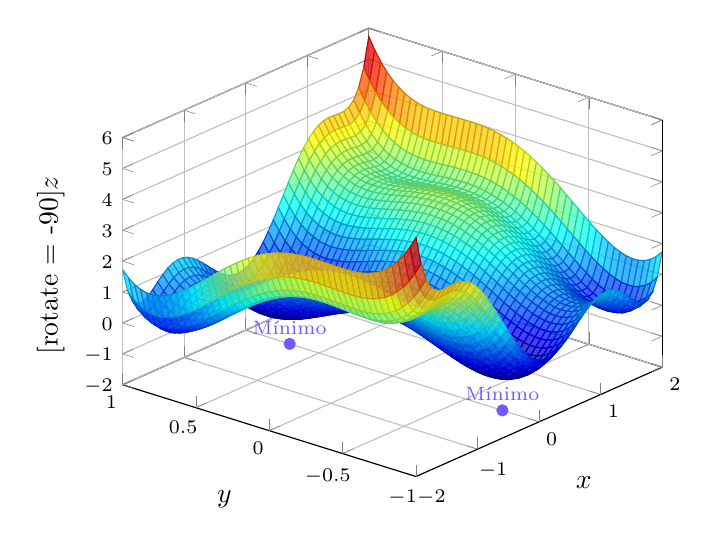
\begin{tikzpicture}
    	\begin{axis}[
    		align =center,
    		view={310}{30},
    		xtick = {2,1,...,-2},
    		ytick = {1,0.5,...,-1},
    		ztick = {6,5,...,-2},
    		xmin=-2,
    		xmax=2,
    		ymin=-1,
    		ymax=1,
    		zmin=-2,
    		zmax=6,
    		ticklabel style = {font = \scriptsize},
    		grid=major,
    		xlabel=$x$,
    		ylabel=$y$,
    		zlabel={[rotate = -90]$z$}     
    		]
    		%some miminum points
    		\addplot3[mark=*,morados,point meta=explicit symbolic,nodes near coords] 
    		coordinates {(0,0.7,-2)[{\scriptsize Mínimo}]};
    		
    		\addplot3[mark=*,morados,point meta=explicit symbolic,nodes near coords] 
    		coordinates {(0,-0.75,-2)[{\scriptsize Mínimo}]};
    		
    		\addplot3 [
    		surf,
    		colormap/jet,
    		shader=faceted,
    		fill opacity=0.75,
    		samples=50,
    		domain=-2:2,
    		y domain=-1:1
    		] {(4-2.1*x^2+x^4/3)*x^2+x*y+(-4+4*y^2)*y^2};
    		
    	\end{axis}
    \end{tikzpicture}
\end{figure}

























\subsubsection{Regularización L1 y L2}
\label{ap:L1L2sec}

La regularización son técnicas utilizadas en aprendizaje automático para evitar un modelo sobre ajuste (\ti{overfitting}) los datos de entrenamiento. Esto ocurre cuando el modelo predice, por lo general, de manera correcta los datos de entrenamiento, pero es incapaz de hacer buenas estimaciones hacia datos con los que no ha entrenado. Si ocurre esto, implica que el modelo tiene una varianza alta (resultados muy distintos ante \ti{inputs} distintos). Por tanto, lo ideal, es encontrar un punto, en el cual, el modelo generado sea capaz de predecir datos de una manera correcta (\ti{low bias}) al mismo tiempo que sea robusto ante distintos datos, i.e. que generalice bien (\ti{low variance}). A esto se le conoce como \ti{Bias-Variance Trade off}. Véase figura \ref{bias_var}.

\begin{figure}[H]
    \centering
    \includegraphics[width = 0.8\textwidth]{imgs/bias_variance.jpg}
    \caption{Error-Varianza. \scriptsize{Fuente: \url{https://aprendeia.com/bias-y-varianza-en-machine-learning/}}}
    \label{bias_var}
\end{figure}

Las técnicas de regularización buscan generar un modelo simple que sea capaz de generalizar bien. A esto se le conoce como principio de parsimonia o la navaja de Okham \parencite{occam}. 

Aunque haya varias técnicas de regularización, L1 y L2 en concreto, penalizan altos valores de pesos (parámetros) en el modelo generado. Esto es porque valores altos de estos pesos, no solo conducen a un modelo más complejo, sino que también a un modelo con mayor varianza\fnm. Estas dos condiciones conducen a un sobre ajuste en el modelo generado. 
\fnt{Basta con imaginar dos pesos $w_1$ y $w_2$ con valores de $0.1$ (bajo) y $100$ (alto) respectivamente. Si se multiplican dos números $A$ y $B$ ---cuales sean--- a estos dos pesos, la diferencia entre $|w_1A - w_1B|$ siempre será menor que  $|w_2A - w_2B|$, y por ende, $w_1$ (un peso bajo) conduce a una menor varianza.}

Por un lado, L1 (también conocido como LASSO: \ti{Least Absolute Shrinkage and Selection Operator}) penaliza valores altos en los pesos del modelo añadiendo la suma en valor absoluto de estos a la función de coste:
\begin{equation}
    \label{L1}
    J(\theta) = J'(\theta) + \underbrace{\textstyle{\lambda \Sum{j=1}{p}|w_j|}}_{\mathclap{\text{Regularización L1}}}
\end{equation}

\begin{quote}
    En donde:
    \begin{itemize}
        \item $J'(\theta)$ es la función de pérdida definida para el problema, la cual se busca \B{minimizar}.
        \item $\lambda$ es un factor $\in (0,1)$ que indica la fuerza de la penalización: cuanto más cercano a $1$ más fuerte es.
        \item $p$  es el número total de pesos del modelo.
        \item $w_j$ es el valor de un peso en concreto.
        \item $J(\theta)$ es la función de pérdida resultante.
    \end{itemize}
\end{quote}

Como los pesos se pasan a valor absoluto, siempre serán positivos y por tanto siempre añadirán valor a la función de coste $J'(\theta)$. Como está función de coste, el objetivo es minimizarla, se están penalizando valores de pesos altos. 

Por otro lado, L2 (también conocida como \ti{Ridge}) también penaliza valores altos de los pesos del modelo, pero en vez de aplicar el valor absoluto, aplica el cuadrado de estos. De  esta manera, al igual que con el valor absoluto, siempre son positivos, y por ende, el valor de los pesos siempre suma a la función de coste.

\begin{equation}
    \label{L2}
    J(\theta) = J'(\theta) + \underbrace{\textstyle{\lambda \Sum{j=1}{p} {w_j}^2}}_{\mathclap{\text{Regularización L2}}}
\end{equation}

En la ec. \ref{L2}, las variables tienen en mismo significado que en la ec.\ref{L1}

Se llaman L1 y L2 porque aplican las normas L1 (o norma Manhattan) y L2 (o norma euclidiana) de matemáticas\fnm.
\fnt{La regularización L2 es en realidad la norma L2 sin la raíz cuadrada.}

Mientras L1 tiende a asociar un valor de $0$ a aquellos pesos irrelevantes en el modelo y mantener sólo aquellos que realmente importan, L2, por el otro lado tiende a mantener todos los pesos más o menos equilibrados con un valor próximo a cero. En algoritmos como regresión lineal, en donde cada peso está asociado a una variable del modelo, esto tiene una interpretación muy clara:
\begin{itemize}
    \item Si se sospecha que varias variables del modelo son irrelevantes y/o no están correladas entre sí, se recomienda emplear L1 ---pues asignará un valor de $0$ a aquellos pesos asociados con variables irrelevantes---.
    \item Por el contrario, si se sospecha que varias variables influyen en el modelo y/o están correladas entre sí, se recomienda usar L2.
\end{itemize}

Sin embargo, en otros algoritmos, esta interpretación no es tan clara y es posible usar ambos a la vez: como hace \B{XGBoost}.

La razón por la que L1 conduce a determinados pesos a ser $0$ y L2 a tener valores bajos, se puede ver muy bien si se grafican las funciones $|x|$, i.e. L1 y $x^2$, i.e. L2. 

\begin{figure}[H]
    \centering
    \begin{tikzpicture}[scale = 5]
      % Ejes
      \draw[->] (-1.3,0) -- (1.3,0) node[right] {$x$};
      \draw[->] (0,-0.25) -- (0,1.3) node[above] {$y$};
      
      % Marcas en el eje x
      \foreach \x in {-1, -0.6, -0.2, 0.2, 0.6, 1}
        \draw (\x,0.75pt) -- (\x,-0.75pt) node[below] {$\x$};
      
      % Función |x|
      \draw[azulos, domain=-1:1, smooth, thick] plot (\x, {abs(\x)}) node[right] {};
      
      % Función x^2
      \draw[morados, domain=-1:1, smooth, thick] plot (\x, {\x*\x}) node[above right] {};

      % Líneas verticales
      \draw[dashed] (-0.2,0) -- (-0.2,0.5);
      \draw[dashed] (0.2,0) -- (0.2,0.5);

      %llaves
      \draw [black, thick, decorate, decoration={brace,amplitude=1.5pt,mirror,raise=5pt}] (0.25,0.0075) -- (0.25,0.06) node [black,midway,right,xshift=0.6cm] {};
      \draw [black, thick,  decorate, decoration={brace,amplitude=2pt,mirror,raise=5pt}] (0.3,0.0075) -- (0.3,0.22) node [black,midway,right,xshift=0.6cm] {};
      % Leyenda
      \draw[azulos, thick] (-0.5,1.3) -- (-0.4,1.3) node[right] {$|x|$};
      \draw[morados, thick] (0.4,1.3) -- (0.5,1.3) node[right] {$x^2$};
    \end{tikzpicture}
    \caption{Gráficas $|x|$ y $x^2$.}
    \label{L1L2}
\end{figure}

Dentro del contexto en el que los pesos están normalizados y, por tanto, sus valores $\in [-1, 1]$, en la gráfica \ref{L1L2} se puede ver cómo incrementos en el eje $x$ no tienen un impacto muy significativo en la imagen  de $x^2$; pero en cambio, sí que lo tienen en la imagen de la función $|x|$. Esto se traduce en que, mientras en L1 si hay una gran diferencia entre que un peso se aproxime mucho a cero -----a si no lo hace---, en $x^2$ no importa tanto. En \ref{L1L2} se ha puesto el ejemplo de $x = \pm 0.2$, pero esto mismo se puede aplicar a cualquier $x \in (-1,1)$.


\subsection{Desvanecimiento del gradiente y gradiente explosivo}
\label{ap:grad}
El mecanismo por el que las redes neuronales aprenden, es a través de la optimización de sus pesos. Estos pesos se actualizan después de un determinado número de entrenamientos (se especifica con el \ti{batch size}). La optimización de estos pesos se hace mediante el algoritmo de \B{Backpropagation} \parencite{bp}.

Este algoritmo revolucionó el campo de la inteligencia artificial. Se basa en la regla de la cadena para la optimización de pesos. De manera muy simplificada, esta regla de la cadena son multiplicaciones. En muchas ocasiones, la actualización de un peso implica muchas multiplicaciones\footnote{miles de multiplicaciones.}.


Ahora, el problema del \B{desvanecimiento del gradiente} surge cuando muchos de estos valores que se están multiplicando  $\in (-1, 1)$. Cuando se multiplican muchas veces (miles de veces) números $\in (-1,1)$, el resultado que se obtiene es un número extremadamente pequeño. Luego este peso que se está tratando de actualizar, no lo hace de una manera eficiente ---pues se actualiza en una cantidad ínfima---.

Por el contrario, el problema del \B{gradiente explosivo} se da cuando la mayoría de estas multiplicaciones $\notin (-1,1)$. El resultado de multiplicar muchas veces números $\notin (-1,1)$ da lugar a un número muy grande. Luego el peso que se está tratando de actualizar lo hace de manera muy brusca y no llega a converger a un valor óptimo.

Las RNN, por su naturaleza, pueden caer en estos problemas.

\subsection{Transformers: origen y explicación}
\label{ap:trans}

Como se ha mencionado, los Transformers tienen su origen en el campo del procesamiento del lenguaje natural. Este campo ha sido de especial interés a lo largo del siglo XXI, ya sea para generar texto, generar \ti{chatbots}, traducción, resúmenes, etc. 

Ahora, las redes neuronales, no entienden de palabras, entienden de números. Para pasarlas a números, lo que se hizo fue \ti{one-hot encoding}. Es decir, un vector de tantas posiciones como palabras tuviera el diccionario. Cada posición hace referencia a una palabra del diccionario. Entonces, cada palabra es un vector de todos ceros, menos un uno en su posición correspondiente. 


Para comprimir toda esta información, este vector se convierte en otro de menor dimensionalidad. A esto se le conoce como \ti{embedding} \parencite{word2vecOriginal} \parencite{word2vecExtension}. De esta manera, se obtenía información característica de una palabra en un vector mucho menor. Dicho vector es muy característico, pues palabras con relación entre sí (e.g. enero y febrero)  tienen asignados vectores muy parecidos. Para poder visualizar esto, se puede comprimir esta información de cada palabra en un vector de tres dimensiones, y el resultado es el siguiente:

\begin{figure}[H]
    \centering
    \includegraphics[scale = 0.5]{imgs/word2vec.png}
    \caption{Palabras representadas en vectores de tres dimensiones. Cada punto es el final del vector, i.e. cada palabra. \scriptsize{Fuente: \url{https://projector.tensorflow.org/}}}
    \label{word2vec}
\end{figure}

Con las palabras expresadas en números, había que encontrar una red neuronal para entrenarla y las RNN\fnm, al ser redes neuronales con \ti{memoria}, fueron la solución \parencite{seq2seq}, \parencite{rnnEncoderDecoder}. Sin embargo, las RNN sufrían el problema de memoria a largo plazo, muy importante en las secuencias de palabras como se puede ver en el siguiente ejemplo:
\fnt{Cabe destacar  que RNN también engloba a las redes neuronales LSTM y GRU.}

\begin{figure}[H]
    \centering
    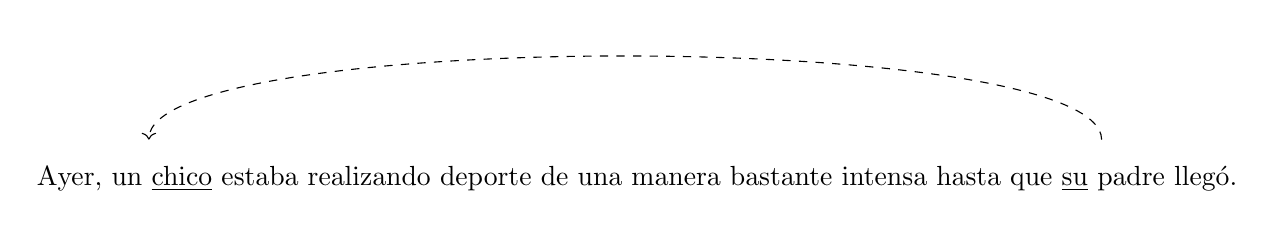
\begin{tikzpicture}
        % Sodes
        \node (inicio) {Ayer, un \ul{chico} estaba realizando deporte de una manera bastante intensa hasta que \ul{su} padre llegó.};
        
         % Bent Arrow
        \draw[->, dashed, bend right, looseness = 0.3] (5.9,0.5) to[out=270, in=270] (-6.2,0.5) node[midway, above] {};
    \end{tikzpicture}
    \caption{Ejemplo, rentención de memoria en texto. La palabra \ti{su} hace referencia a una palabra muy anterior a ella (\ti{chico}).}
\end{figure}

Para solventar el problema de las RNN se añadió a estas el concepto de atención ---i.e. RNN + atención---\parencite{rnnPlusAttention}. Este tipo de redes supusieron el estado de arte en el campo de NLP durante mucho tiempo \parencite{rnnAttentionMejorada1} \parencite{rnnAttentionMejorada2} \parencite{rnnAttentionMejorada3}.

Pese a que se obtenían buenos resultados con estas redes neuronales, sufrían de que tardaban mucho tiempo en entrenarse. Esto es porque este entrenamiento se realizaba de manera secuencial. Es decir, se iba procesando palabra por palabra, lo que resultaba en un entrenamiento muy costoso.

En 2017, surge una nueva red neuronal: Los Transformers \parencite{transformers}. Los creadores de esta red neuronal, se dieron cuenta de que en el algortimo mencionado anteriormente (RNN + atención), la RNN no hacía falta, y que con la atención era suficiente. Esta es la razón del nombre de la publicación: \ti{Atention is all you need}. Esta red neuronal cambió el campo de NLP ---y posteriormente muchos otros cuando utilizó Transformer en ellos: e.g. imágenes---. No sólo obtenían mejores resultados que sus antecesores, sino que también su entrenamiento no era secuencial; sino que era paralelizable. Es decir, que esta red neuronal entrena con todos los datos disponibles al mismo tiempo convirtiéndolo más eficiente también. Su arquitectura es la siguiente:

\begin{figure}[H]
    \centering
    \begin{tikzpicture}
        \node {\includegraphics[scale=0.9]{imgs/tranformer_arquitecture.png}};
        \draw [black, ultra thick, decorate, decoration={brace,amplitude=10pt,mirror,raise=5pt}] (-3.5,1.1) -- (-3.5, -2.6) node [black,midway,left,xshift=-0.6cm] {Encoder};
        \draw [black, ultra thick, decorate, decoration={brace,amplitude=10pt,mirror,raise=5pt}] (3.75,-2.3) -- (3.75,2.7) node [black,midway,right,xshift=0.6cm] {Decoder};
    \end{tikzpicture}
    \caption{Arquitectura del Transformer original. \scriptsize{Fuente: \parencite{transformers}}}
    \label{transformer}
\end{figure}

Sus autores, denominan a esta arquitectura como \ti{simple}. Por muy \ti{trivial} que parezca, se va a proceder sus partes. Se va a empezar explicando la parte izquierda primero; luego la derecha es muy parecida.

\subsubsection{Embedding y codificador posicional}

\bigskip

\begin{figure}[H]
    \centering
    \includegraphics{imgs/trans_arq_1.png}
    \caption{Parte izquierda: embedding y encoding posicional. \scriptsize{Fuente: \parencite{transformers}}}
    \label{inputs_encoder}
\end{figure}
Los \ti{inputs} (figura \ref{inputs_encoder}), estando dentro el contexto de NLP, son secuencias (oraciones). Estas secuencias están formadas por palabras (denominadas como \ti{tokens}\fnm). Las palabras, como ya se ha mencionado con anterioridad, es necesario transformarlas en valores numéricos para poder ser analizadas y procesadas por una red neuronal. A esta transformación se la conoce como \ti{embedding} y su resultado es un vector numérico\fnm\ con la información de la palabra. La dimensión de este vector será consistente a lo largo de la red neuronal como se verá más adelante.
\fnt{En realidad un \ti{token} puede ser una letra o alguna otra división de texto. Esto depende de 
la segmentación que se quiera hacer. Por lo general, será una palabra.}
\addtocounter{footnote}{1}
\fnt{En el \ti{paper}, este vector tiene 512 dimensiones. $v \in \mathbb{R}^{d_{model}}, \quad d_{model} = 512$.}

El \B{codificador posicional} (figura \ref{inputs_encoder}), probablemente sea de lo más importante en la arquitectura. Como ya se ha dicho, esta red neuronal no es secuencial, y entrena con todas las palabras al mismo tiempo. Por esto, es necesario añadir algo de información al vector embedding para indicar la posición de la palabra en la oración ---pues esta es muy importante\fnm---. Para ello, se genera un nuevo vector ---de igual dimensión al embedding--- que se sume al vector embedding. Ideas triviales, como la de que dicho vector sea todo ceros, menos un uno en la posición que ocupe la palabra en la oración no sirven; pues si la oración tiene muchas palabras, la suma daría lugar a un vector de valores muy altos, añadiendo de esta manera complejidad al entrenamiento. Otra idea que tampoco sirve es la de asignar un porcentaje ($pos/pos\_totales$) a la posición de la palabra; pues si dos oraciones, por ejemplo, tienen 2 y 4 palabras respectivamente, la primera palabra de la primera oración y la segunda palabra de la segunda oración tendrían el mismo porcentaje (0.5).
\fnt{No es lo mismo la oración: \ti{Me río en el baño}; que la de: \ti{Me baño en el río}.}

La solución pues, pasa por hacer que este vector sea sinusoidal\fnm, con una \B{frecuencia distinta para cada posición}. La idea intuitiva de representar un orden con frecuencia, se puede ver con la codificación binaria \parencite{binary_frequency} (véase tablas \ref{cod_binaria} y \ref{frec_binaria}).
\begin{table}[H]
    \centering
    \begin{tabular}{c c c c c c c c}
        0: &  0 & 0  & 0 \\
        1: &  0 & 0  & \cellcolor{moradcl}1 \\
        2: &  0 & \cellcolor{moradcl}1  & 0 \\
        3: &  0 & \cellcolor{moradcl}1  & \cellcolor{moradcl}1 \\
        4: &  \cellcolor{moradcl}1 & 0  & 0 \\
        5: &  \cellcolor{moradcl}1 & 0  &\cellcolor{moradcl} 1 \\
        6: &  \cellcolor{moradcl}1 & \cellcolor{moradcl}1  & 0 \\
        7: &  \cellcolor{moradcl}1 & \cellcolor{moradcl}1  & \cellcolor{moradcl}1 \\
        \end{tabular}
    \caption{Patrón en codificación binaria}
    \label{cod_binaria}
\end{table}

En la tabla \ref{cod_binaria}, se puede ver un patrón alternante entre 0's y 1's en cada columna. Si esto, se pasa del mundo discreto al mundo continuo, queda de la siguiente manera (véase tabla \ref{frec_binaria}).
\begin{table}[H]
    \centering
    \begin{tabular}{c c c c c c c c}
        0 & 1 & 0 & 1 & 0 & 1 & 0 & 1 \\
        0 & 0 & 1 & 1 & 0 & 0 & 1 & 1 \\
        0 & 0 & 0 & 0 & 1 & 1 & 1 & 1 \\
        \begin{tikzpicture}[overlay, remember picture, scale=0.5]
            \draw[red,domain=-1.2:9,samples=250, thick] plot (\x+0.85,{sin(\x*142)+7});
        \end{tikzpicture}
        \begin{tikzpicture}[overlay, remember picture, scale=0.5]
            \draw[orange,domain=-2.5:7.5,samples=250, thick] plot (\x+1.9,{sin(\x*71)+4.5});
        \end{tikzpicture}
        \begin{tikzpicture}[overlay, remember picture, scale=0.5]
            \draw[morados,domain=-5:5,samples=250, thick] plot (\x+4.2,{sin(\x*35.5)+2.40});
        \end{tikzpicture}
    \end{tabular}
    \caption{Tabla \ref{cod_binaria} traspuesta: Frecuencia para número binarios.}
    \label{frec_binaria}
\end{table}

En el \ti{paper}, esta es una fórmula matemática más compleja utilizando senos para posiciones pares y cosenos para las impares, pero la idea es la misma: tener una frecuencia única para cada posición. Además, esta codificación tiene una ventaja, y es que los autores hipotetizan que de esta manera, el modelo es más robusto a trabajar con longitudes de secuencias que no ha visto en el entrenamiento.

En resumen, esta parte de la arquitectura recibe la \B{secuencia de entrada}. Esta secuencia está compuesta de palabras y cada palabra se transforma en un vector de $512$ dimensiones. Por tanto, lo que se pasa a la siguiente capa es una matriz $E$ de dimensiones $[S, 512]$ siendo $S$ el número de palabras de la secuencia y $512$ la longitud del vector de  cada palabra.  Es importante remarcar que esta dimensión de salida es consistente a lo largo de todo el proceso.

\subsubsection{Encoder}
\label{encoder}
El \ti{Encoder} se compone de seis capas. Estas capas son repeticiones de la anterior, i.e. son todas iguales. El objetivo de estas capas es que, dada una palabra de la oración, a qué otras palabras hay que prestar \B{atención} de la oración. A esto se le conoce como \ti{self-attention}.

 Esta información será vital para luego pasársela al  \ti{Decoder} ---que es quien se encargará de generar la salida (texto) del modelo---.

\subsubsubsection{Atención Encoder}
Junto con la codficación posicional, esto es lo más importante del algoritmo.
\begin{figure}[H]
    \centering
    \includegraphics[scale=1.1]{imgs/trans_arq_2.png}
    \begin{tikzpicture}[overlay]
        \draw[->, black, ultra thick] (2,1.25) -- (0,1.25);
        \draw[->, black,  thick] (-5.75,2.15) -- (-4.25,2.15);
        \node[left] at (-6, 2.15) {$N = 6$\footnotesize{: nº capas Encoder}};
    \end{tikzpicture}
    \caption{Atención múltiple. \scriptsize{Fuente: \parencite{transformers}}}
\end{figure}

La atención consiste en que el algoritmo sepa que, dada una palabra de la oración, a qué otras palabras debe prestarle atención. Por ejemplo, en la oración \ti{El chico juega}, el Transformer, en el verbo, debe prestar atención a la palabra \ti{chico} para poder conjugarlo bien.

Para conseguir esta atención, hay tres redes neuronales involucradas: \ti{Query} ($Q$), \ti{Key} ($K$) y \ti{Value} ($V$). Las tres redes neuronales se van a encargar de generar un vector ---con distintos propósitos--- por cada palabra en la secuencia de entrada (todos estos vectores tienen la misma dimensionalidad que el vector \ti{embedding}, i.e. $d_{model} = 512$). 

Desarrollando un poco más esto, el vector de cada palabra que genera la red neuronal $Q$ describe, por decirlo de alguna manera, las cualidades que debe cumplir otra palabra de la secuencia para que la palabra en cuestión le preste atención. El vector que genera $K$ define una descripción de dicha palabra. En otras palabras, $Q$ genera un vector de las características que busca una palabra para prestar atención a otra; mientras que $K$ genera un vector de las características de cada palabra. Por tanto, las redes $Q$ y $K$ trabajan en conjunto para generar el vector de atención. 

Una manera de ver esto de manera más visual es pensar como que cada palabra de la oración tiene una llave (vector generado por $K$) y un candado (vector generado por $Q$). Cogiendo el ejemplo de antes, esto se vería así:

\begin{table}[H]
    \centering
    \setlength{\tabcolsep}{2cm} % Ajusta el espacio entre las columnas
    \begin{tabular}{cc}
        El \hspace{0.075cm} \raisebox{-0.25cm}{\includegraphics[height=0.6cm]{imgs/key}} &  \raisebox{-0.25cm}{\includegraphics[height=0.9cm]{imgs/query}} El   \\
        chico \hspace{0.075cm} \raisebox{-0.25cm}{\includegraphics[height=0.6cm]{imgs/key}} & \raisebox{-0.25cm}{\includegraphics[height=0.9cm]{imgs/query}} \hspace{0.075cm}chico \\
        juega \raisebox{-0.25cm}{\includegraphics[height=0.6cm]{imgs/key}} & \raisebox{-0.25cm}{\includegraphics[height=0.9cm]{imgs/query}}  juega
    \end{tabular}
    \caption{Representación gráfica de vector \ti{key} de cada palabra (columna de la izquierda) y el vector \ti{query} de cada palabra (columna de la derecha).}
    \label{QK}
\end{table}

Entonces, cada vector \ti{query} de cada palabra, se compara con cada vector \ti{key} de cada palabra. En decir, se está comparando las características que busca cada palabra (\ti{query}) con la descripción del resto de palabras en la oración (\ti{key}). 
\begin{table}[H]
    \centering
    \setlength{\tabcolsep}{2cm} % Ajusta el espacio entre las columnas
    \begin{tabular}{cc}
        El \raisebox{-0.25cm}{\includegraphics[height=0.6cm]{imgs/key}} &  \raisebox{-0.25cm}{\includegraphics[height=0.9cm]{imgs/query}} El   \\
        chico \raisebox{-0.25cm}{\includegraphics[height=0.6cm]{imgs/key}} & \raisebox{-0.25cm}{\includegraphics[height=0.9cm]{imgs/query}} chico \\
        juega \raisebox{-0.25cm}{\includegraphics[height=0.6cm]{imgs/key}} & \raisebox{-0.25cm}{\includegraphics[height=0.9cm]{imgs/query}} juega
    \end{tabular}
    \begin{tikzpicture}[overlay, remember picture]
        % Flechas rectas
        \draw[->, moradmed, dashed] (-4,1) -- (-7.7,1);
        \draw[->, morados, dashed] (-4,1) -- (-7.7,0);
        \draw[->, moradcl, dashed] (-4,1) -- (-7.7,-0.9);
    \end{tikzpicture}
    \caption{Comparación entre características de la palabra \ti{El} con la descripción del resto de palabras.}
    \label{QK2}
\end{table}

Esto se hace con todas las palabras de la oración. Quizá se vea de  manera clara con un ejemplo del propio artículo. Véase figura \ref{att_seq}:

\begin{figure}[H]
    \centering
    \includegraphics[scale = 0.35]{imgs/sequence_attention.png}
    \caption{Ejemplo de \ti{self-attention} entre todas las palabras de una secuencia. Cuanto más oscuro es el color, más atención le presta una palabra a la correspondiente.\scriptsize{Fuente: \parencite{transformers}}}
    \label{att_seq}
\end{figure}
De esta manera, si ambos vectores \ti{query} y \ti{key} son parecidos, quiere decir que las características que busca una palabra $A$ son parecidas a la descripción de otra palabra $B$; lo que indica que la palabra $A$ debe prestar atención a $B$. Para saber si dos vectores son parecidos, se emplea el producto escalar: $|Q| \cdot |K| \cdot \cos{\theta}$. Véase la figura \ref{prod_esc}.

\begin{figure}[H]
    \centering
    \begin{subfigure} % Cambia el ancho a 0.48\textwidth
        \centering
        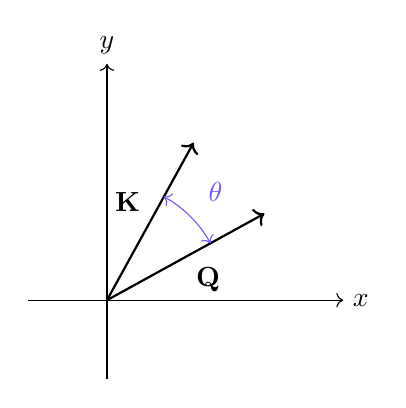
\begin{tikzpicture}
            % Ejes coordenados
            \draw[->] (-1,0) -- (3,0) node[right] {$x$};
            \draw[->] (0,-1) -- (0,3) node[above] {$y$};
            
            % Vector 1
            \draw[->,black,thick] (0,0) coordinate (a) -- (2,1.1) coordinate (b) node[midway, below right] {$\mathbf{Q}$};
            
            % Vector 2
            \draw[->,black,thick] (0,0) -- (1.1,2) coordinate(c) node[midway, above left] {$\mathbf{K}$};
        
            \pic [draw, morados, <->,
              angle radius = 15mm,
              angle eccentricity=1.3, 
              "$\theta$"] {angle = b--a--c};
        \end{tikzpicture}
    \end{subfigure} \hspace{3cm}
    \begin{subfigure} % Cambia el ancho a 0.48\textwidth
        \centering
        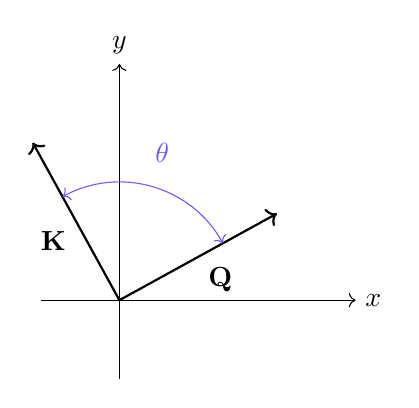
\begin{tikzpicture}
            % Ejes coordenados
            \draw[->] (-1,0) -- (3,0) node[right] {$x$};
            \draw[->] (0,-1) -- (0,3) node[above] {$y$};
            
            % Vector 1
            \draw[->,black,thick] (0,0) coordinate (a) -- (2,1.1) coordinate (b) node[midway, below right] {$\mathbf{Q}$};
            
            % Vector 2
            \draw[->,black,thick] (0,0) -- (-1.1,2) coordinate(c) node[midway, below left] {$\mathbf{K}$};
        
            \pic [draw, morados, <->,
              angle radius = 15mm,
              angle eccentricity=1.3, 
              "$\theta$"] {angle = b--a--c};
        \end{tikzpicture}
    \end{subfigure}
    \caption{Visualización entre ángulo de vectores parejos (izquierda) y vectores disparejos (derecha).}
    \label{prod_esc}
\end{figure}
Como $cos (\theta = 0^\circ) = 1$ y $cos (\theta = 180^\circ) = -1$, de la figura \ref{prod_esc} se deduce  que cuanto mayor sea este producto escalar, más parecidos serán estos vectores

Ahora, como el Transformer realiza todo esto de manera paralela, se puede pensar en $Q$ y en $K$ como matrices de dimensión $[S, 512]$, en donde cada fila de cada una de las matrices corresponde con el vector cuestión de cada palabra. Las matrices $Q$ y $K$ son multiplicadas respectivamente por las matrices $W^Q$ y $W^K$ (ambas de dimensión $[512, 64]$ con el objetivo de proyectar $Q$ y $K$ a matrices $Q'$ y $K'$ de dimensión $[S, 64]$\fnm. Se procede pues, a multiplicar las matrices $Q'$ y $K'$ para obtener la \B{matriz de pesos de atención}. Para ello, hay que trasponer la matriz: $K \rightarrow K^T$:
\fnt{Esto está mal explicado en muchos sitios, en donde explican que Q es el resultado de multiplicar la matriz $E$ por la matriz $W^Q$. Lo mismo con las matrices $K$ y $V$ respectivamente. En el \ti{paper} no se indica nada de eso.}
\begin{figure}[H]
    \centering
    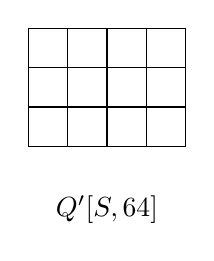
\begin{tikzpicture}[baseline=(current bounding box.center)]
        % Definición de las coordenadas y dibujo de los cuadrados
        \foreach \x in {0,1,2,3} {
            \foreach \y in {0,1,2} {
                \draw (\x*0.5,\y*0.5) rectangle ++(0.5,0.5);
            }
        }
        % Texto debajo de la primera matriz
        \node[below] at (1,-0.5) {$Q'[S,64]$};
    \end{tikzpicture}
    \quad \raisebox{0.5cm}{$\times$} \quad % Espacio entre las imágenes
    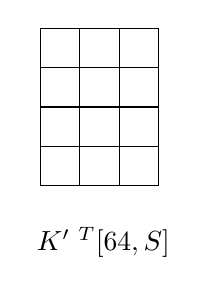
\begin{tikzpicture}[baseline=(current bounding box.center)]
        % Definición de las coordenadas y dibujo de los cuadrados
        \foreach \x in {0,1,2} {
            \foreach \y in {0,1,2,3} {
                \draw (\x*0.5,\y*0.5) rectangle ++(0.5,0.5);
            }
        }
        % Texto debajo de la segunda matriz
        \node[below] at (0.8,-0.4) {$K'\hspace{3pt}^T[64,S]$};
    \end{tikzpicture}
    \qquad \raisebox{0.5cm}= \qquad % Espacio entre las imágenes
    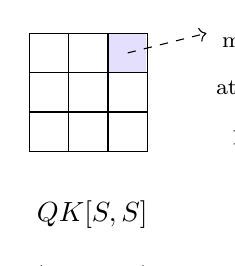
\begin{tikzpicture}[baseline=(current bounding box.center), yshift=0.5cm]
    % Definición de las coordenadas y dibujo de los cuadrados
        \foreach \x in {0,1,2} {
            \foreach \y in {0,1,2} {
                \draw (\x*0.5,\y*0.5) rectangle ++(0.5,0.5);
            }
        }
        % Colorear el último cuadrado de la primera fila
        \fill[moradcl] (1.01,1.01) rectangle ++(0.478,0.478);
        % Texto debajo de la segunda matriz
        \node[below] at (0.8,-0.5) {$QK[S,S]$};
        \draw [decorate,decoration={brace,amplitude=5pt},yshift=0.5mm, overlay]
        (1.45,-1.5) -- (0.15,-1.5) node [black,midway,yshift=-5mm] {\footnotesize \B{Matriz de pesos de atención}};
        % Flecha con texto dividido en tres líneas
        \draw[->, black, dashed] (1.25, 1.25) -- (2.25, 1.5) node[right, overlay, align = center, yshift=-1cm] {\footnotesize{Esta posición (p.e.) de la} \\ \footnotesize{matriz representa el peso de} \\ \footnotesize{atención que le da la primera } \\
        \footnotesize{palabra (primera fila) a la} \\ \footnotesize{última palabra (última}\\
        \footnotesize{columna) de la secuencia}.};
    \end{tikzpicture}
\end{figure}

Esta matriz resultado ($QK$) se divide entre la raíz de la dimensión de las filas de $Q'$\fnm\ ---i.e. $\sqrt{64} = 8$--- y se pasa por una función Softmax: $QK' = Softmax(QK/8)$.  Esto último, hace que la suma total de atenciones que presta una palabra al resto, sea igual a uno. En otras palabras, la suma de los valores de cada fila de $QK'$ da uno. El objetivo de esto es tratar con valores más simples y estandarizados.
\fnt{Esto se hace para evitar problemas de explosión de gradiente, pues la multiplicación entre $Q'$ y $K'$ puede dar lugar a valores numéricos muy grandes.}

Una vez obtenidos los vectores de pesos estandarizados de cada palabra ---filas de la matriz $QK'$---, habrá que multiplicar dichos pesos al vector valor \ti{propio} de cada palabra. La red neuronal $V$ (\ti{Value}) ---que de la misma manera que $Q$ y $K$, es una matriz de dimensión $[S, 512]$--- es la encargada de generar este vector \ti{propio} para cada palabra en la secuencia. De nuevo, al igual que se ha hecho con $Q$ y $K$, $V$ se reduce (proyecta) a una dimensión $[S, 64]$ al ser multiplicada por una matriz de pesos $W^V[512, 64]$. De esta manera:

\bigskip

\begin{figure}[H]
    \centering
    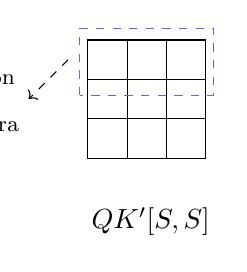
\begin{tikzpicture}[baseline=(current bounding box.center)]
        % Definición de las coordenadas y dibujo de los cuadrados
        \foreach \x in {0,1,2} {
            \foreach \y in {0,1,2} {
                \draw (\x*0.5,\y*0.5) rectangle ++(0.5,0.5);
            }
        }
        % Colorear el último cuadrado de la primera fila
        \draw[morados, dashed] (-0.1,0.8) rectangle (1.6,1.65);
        \draw[->, black, dashed] (-0.25, 1.25) -- (-0.75, 0.75) node[below left, overlay, align = center, yshift=0.5cm] {\footnotesize{vector atención} \\ \footnotesize{primera palabra}};
        % Texto debajo de la segunda matriz
        \node[below] at (0.8,-0.5) {$QK'[S,S]$};
    \end{tikzpicture}
    \quad \raisebox{0.4cm}{$\times$} \quad % Espacio entre las imágenes
    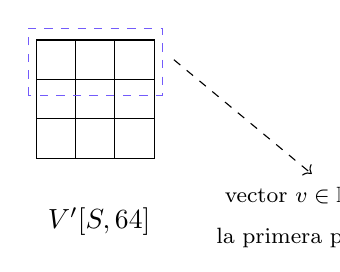
\begin{tikzpicture}[baseline=(current bounding box.center)]
        % Definición de las coordenadas y dibujo de los cuadrados
        \foreach \x in {0,1,2} {
            \foreach \y in {0,1,2} {
                \draw (\x*0.5,\y*0.5) rectangle ++(0.5,0.5);
            }
        }
        \draw[morados, dashed] (-0.1,0.8) rectangle (1.6,1.65);
        \draw[->, black, dashed] (1.75, 1.25) -- (3.5, -0.2) node[below, overlay, align = center] {\footnotesize{vector $v \in \mathbb{R}^S$ de} \\[-0.2em] \footnotesize{la primera palabra}};
        % Texto debajo de la segunda matriz
        \node[below] at (0.8,-0.5) {$V'[S,64]$};
    \end{tikzpicture}
    \qquad \raisebox{0.4cm}{$=$} \qquad % Espacio entre las imágenes
    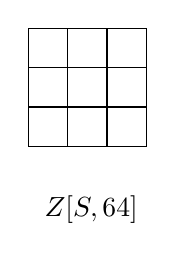
\begin{tikzpicture}[baseline=(current bounding box.center)]
        % Definición de las coordenadas y dibujo de los cuadrados
        \foreach \x in {0,1,2} {
            \foreach \y in {0,1,2} {
                \draw (\x*0.5,\y*0.5) rectangle ++(0.5,0.5);
            }
        }    
        \node[below] at (0.8,-0.5) {$Z[S,64]$};
    \end{tikzpicture}
\end{figure}
\bigskip
\bigskip
Una manera más intuitiva de entender cómo están formadas las filas de la matriz $QKV$ es la siguiente:

\bigskip

\hspace*{1.5cm}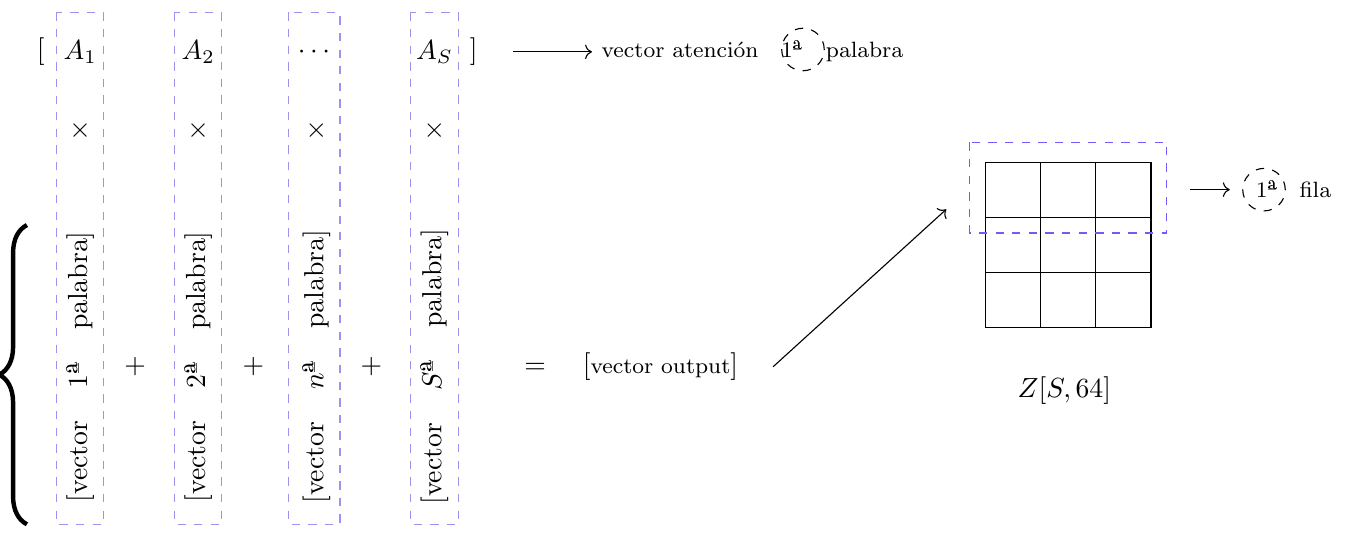
\begin{tikzpicture}[baseline=(current bounding box.center), xshift = 15cm]
    % Vector superior
    \node at (1,0) {$[$}; % Add [
    \foreach \i/\content in {1/A_1, 2/A_2, 3/\cdots, 4/A_S} {
        \node at (\i*1.5,0) {$\content$}; 
        \node at (\i*1.5,-1) {$\times$}; 
        \pgfmathparse{int(\i)} % Evaluate the current value of \i as an integer
        \ifnum\pgfmathresult=3
            \node[rotate=90] at (\i*1.5,-4) {[vector \hspace{5pt} $n$ª \hspace{5pt} palabra]};
        \else
            \ifnum\pgfmathresult=4
                \node[rotate=90] at (\i*1.5,-4) {[vector \hspace{5pt} $S$ª \hspace{5pt} palabra]};
            \else
                \node[rotate=90] at (\i*1.5,-4) {[vector \hspace{5pt} \iª \hspace{5pt} palabra]}; 
            \fi
        \fi
    }
    \begin{scope}[overlay]
    \draw [black, ultra thick, decorate, decoration={brace,amplitude=10pt,mirror,raise=5pt}] (1,-2.2) -- (1, -6) node [black,midway,left,xshift=-0.2cm, overlay] {
        \begin{minipage}{1.5cm} % Ancho del minipage
            \centering % Centrar el texto dentro del minipage
            \small{filas} \\
            \small{$V$}
        \end{minipage}
    };
    \end{scope}
    \node at (6.5,0) {$]$};  
    % Sodos +
    \foreach \x in {2.2, 3.7, 5.2} {
        \node at (\x, -4) {+};
    }
    
    \draw[->, black] (7, 0) -- (8, 0) node[right, overlay,] {\footnotesize{vector atención \hspace{2.5pt} 1ª \hspace{2.5pt} palabra}};
    \draw[moradmed, dashed, overlay] (1.2,0.5) rectangle (1.8, -6);
    \draw[moradmed, dashed, overlay] (2.7,0.5) rectangle (3.3, -6);
    \draw[moradmed, dashed, overlay] (4.15,0.5) rectangle (4.8, -6);
    \draw[moradmed, dashed, overlay] (5.7,0.5) rectangle (6.3, -6);
    \node at (8.5,-4) {= $\quad [\text{\footnotesize{vector output}}]$};
    
   

   \begin{scope}[overlay, xshift=13cm, yshift=-3.5cm]
        \foreach \x in {0,1,2} {
            \foreach \y in {0,1,2} {
                \draw (\x*0.7,\y*0.7) rectangle ++(0.7,0.7); 
            }
        }
        \draw[morados, dashed] (-0.2,2.35) rectangle (2.3,1.2);
        \node[below] at (1,-0.5) {$Z[S,64]$};
    \end{scope}

    \draw[->, black] (10.3, -4) -- (12.5, -2);
    \draw[->, black] (15.6, -1.75) -- (16.1, -1.75) node[pos = 0.92mm]{\footnotesize{1ª \hspace{5pt}fila}};
    \draw[dashed] (16.535,-1.75) circle (0.27cm);
    \draw[dashed] (10.68,0.03) circle (0.27cm);
\end{tikzpicture}

\bigskip

\bigskip

Hasta este punto, se ha hecho lo que se llama como \ti{atención de producto escalar escalado}. Ahora, una sola atención puede no ser suficiente; es decir, puede ser necesario ---y lo es en la mayoría de casos--- prestar atención a más que simples palabras. Por ejemplo, en la frase \ti{Me gusta la lasaña} hay que poner el foco en más de una atención (véase figura \ref{mult_atenc}).
\begin{figure}[H]
    \centering
    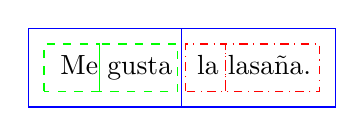
\begin{tikzpicture}
        \node {Me gusta \hspace{0.2cm}la lasaña.};
        \draw[green, dashed] (-1.8,-0.3) rectangle (-1.1,0.3);
        \draw[green, dashed] (-1.1, -0.3) rectangle (-0.1, 0.3);
        \draw[red, dash dot] (0, -0.3) rectangle (0.5, 0.3);
        \draw[red, dash dot] (0.5, -0.3) rectangle (1.7, 0.3);
        \draw[blue] (-2, -0.5) rectangle (-0.05, 0.5);
        \draw[blue] (-0.05, -0.5) rectangle (1.9, 0.5);
    \end{tikzpicture} 
    \caption{Ejemplo. de atención múltiple.}
    \label{mult_atenc}
\end{figure}

\bigskip 

En la figura \ref{mult_atenc} se puede ver cómo hay relación entre las palabras \ti{Me} y \ti{gusta}; así como entre las palabras \ti{la} y \ti{lasaña}. Pero también hay una relación entre \ul{\ti{Me gusta}} y \ul{\ti{la lasaña}}. Es por esto que es necesario tener en cuenta varias dimensionalidades de la atención. Para ello, las matrices $Q$, $K$, $V$ se repiten $h = 8$ veces en cada capa (véase figura \ref{mult_head}).

\begin{figure}[H]
    \centering
    \includegraphics[scale = 0.7]{imgs/trans_arq_2.2.png}
    \begin{tikzpicture}[overlay]
        \draw[->, black, ultra thick] (1.75,1.85) -- (-0.3,1.85) node[pos=+0.3, right, align = center] { 
        \begin{minipage}{6cm}% Ancho del minipage
            \centering % Centrar el texto dentro del minipage
            \footnotesize{matrices $W^V, W^K, W^Q$} \\
            \footnotesize{respectivamente}
        \end{minipage}
    };
        \draw[->, black, ultra thick] (1.75,5.5) -- (-2,5.5) node[pos=0.2, right, align = center] {
        \begin{minipage}{6cm}% Ancho del minipage
            \centering % Centrar el texto dentro del minipage
            \footnotesize{matriz $W^O$ explicada} \\
            \footnotesize{a continuación}
        \end{minipage}
    };
        \draw[->, black,  thick] (1,3.1) -- (0,3.1) node[pos=-0.05, right] {\footnotesize{= 8}};
    \end{tikzpicture}
    \caption{Atención llevada a más de una dimensionalidad. \scriptsize{Fuente: \parencite{transformers}}}
    \label{mult_head}
\end{figure}

De esta manera, se genera una nueva matriz $Z$ por cada dimensión. Cada una de estas matrices se va concatenando a la anterior. Como esto se repite ocho veces, se acaba con un matriz $Z'[S, 64\cdot 8]$. Esta matriz, con el fin de de que tenga el mismo tamaño de entrada que la matriz de entrada en la  capa de entrada ---i.e. $[S,512]$, tamaño de la matriz $E$---, se multiplica por otra matriz de pesos $W^O[64 \cdot 8,512]$. Véase la figura \ref{final_mult_head}.

\begin{figure}[H]
    \centering
    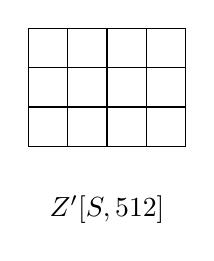
\begin{tikzpicture}[baseline=(current bounding box.center)]
        % Definición de las coordenadas y dibujo de los cuadrados
        \foreach \x in {0,1,2,3} {
            \foreach \y in {0,1,2} {
                \draw (\x*0.5,\y*0.5) rectangle ++(0.5,0.5);
            }
        }
        % Texto debajo de la primera matriz
        \node[below] at (1,-0.5) {$Z'[S,512]$};
    \end{tikzpicture}
    \quad \raisebox{0.5cm}{$\times$} \quad % Espacio entre las imágenes
    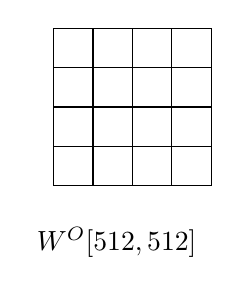
\begin{tikzpicture}[baseline=(current bounding box.center)]
        % Definición de las coordenadas y dibujo de los cuadrados
        \foreach \x in {0,1,2,3} {
            \foreach \y in {0,1,2,3} {
                \draw (\x*0.5,\y*0.5) rectangle ++(0.5,0.5);
            }
        }
        % Texto debajo de la segunda matriz
        \node[below] at (0.8,-0.4) {$W^O[512,512]$};
    \end{tikzpicture}
    \qquad \raisebox{0.5cm}= \qquad % Espacio entre las imágenes
    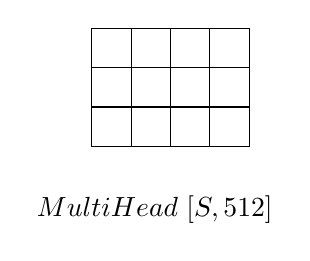
\begin{tikzpicture}[baseline=(current bounding box.center), yshift=0.3cm]
    % Definición de las coordenadas y dibujo de los cuadrados
        \foreach \x in {0,1,2,3} {
            \foreach \y in {0,1,2} {
                \draw (\x*0.5,\y*0.5) rectangle ++(0.5,0.5);
            }
        }
        % Texto debajo de la segunda matriz
        \node[below] at (0.8,-0.5) {$MultiHead\hspace{3pt}[S,512]$};
    \end{tikzpicture}
    \caption{Matriz final de atención.}
    \label{final_mult_head}
\end{figure}

\subsubsubsection{Bloque residual}
\begin{figure}[H]
    \centering
    \begin{tikzpicture}
        \node {\includegraphics[scale=1.1]{imgs/trans_arq_2.png}};
        \draw[->, black, ultra thick] (4,-0.3) -- (2,-0.3);
        \node[right] at (4, -0.3){\footnotesize{$1^{\text{er}}$ \hspace{2pt} bloque residual}};
        \draw[->, black, ultra thick] (4,1.7) -- (2,1.7);
        \node[right] at (4, 1.7){\footnotesize{$2^{\text{\hspace{1pt}ndo}}$ \hspace{2pt} bloque residual}};
    \end{tikzpicture}
    \caption{Ajuste de valores. \scriptsize{Fuente: \parencite{transformers}}}
    \label{bloque_residual}
\end{figure}

El bloque residual \parencite{bloqueResidual} se encarga de ajustar los valores para mejorar el rendimiento del entrenamiento y hacerlo más sencillo. Esto es necesario debido a la gran profundidad que tiene esta arquitectura. En la figura \ref{bloque_residual}, si uno se fija bien, le llegan dos \ti{inputs}: el de la subcapa anterior y el de la anterior a esta. Es decir, al primer bloque residual ---el de más abajo en la figura \ref{bloque_residual}--- recibe la matriz de los \ti{embeddings}\fnm\ y la matriz \ti{MultiHead} (figura \ref{final_mult_head}); ambas con la misma dimensión: $[S, 512]$. El segundo bloque residual, el de más arriba, recibe sin embargo el \ti{output} de este primer bloque residual y el \ti{output} de la red neuronal FFN (\ti{Feed Forward Network}).
\fnt{Cabe recordar que hay $6$ capas en total como las de la figura \ref{bloque_residual}. Es decir, el bloque residual de más abajo de la figura \ref{bloque_residual} recibe la matriz de \ti{embeddings} por ser la primera de las seis capas. En las siguientes, esto no ocurre; recibe el output del \ti{Encoder} de la capa anterior.}

En cualquier caso, \B{el \ti{output} de todas las subcapas es siempre constante: una matriz de dimensiones} $[S,512]$. El bloque residual por tanto, de lo único que se encarga es de sumar las dos matrices que recibe de los dos sub-bloques anteriores y las normaliza. Esto último acelera y simplifica el entrenamiento \parencite{batchNormalization}.

\subsubsubsection{Red de retroalimentación}

\begin{figure}[H]
    \centering
    \begin{tikzpicture}
        \node {\includegraphics[scale=1.1]{imgs/trans_arq_2.png}};
        \draw[->, black, ultra thick] (4,1) -- (2,1);
        \node[right] at (4,1) {\footnotesize{F\hspace{1pt}F\hspace{1pt}N}};
    \end{tikzpicture}
    \caption{F\hspace{1pt}F\hspace{1pt}N. \scriptsize{Fuente: \parencite{transformers}}}
    \label{FFN}
\end{figure}

Lo último por explicar del \ti{Encoder} es la red de retroalimentación (FFN, por sus siglas en inglés). Esta red consiste en una MLP que es aplicada a cada palabra de la secuencia (oración) de manera separada. Esta red neuronal agrega no linealidad\fnm\ al algoritmo, haciendo posible el aprendizaje de relaciones más complejas.

Cabe remarcar que los pesos de estar red neuronal FFN, al igual que el resto de redes neuronales ---i.e. $Q, K, V$ y las matrices de pesos $W$---, son distintos en cada capa.
\fnt{Esto se consigue con las funciones de activación. En este caso de aplica una ReLu $\begin{cases} 
0 & \text{si } x < 0 \\
x & \text{si } x \geq 0
\end{cases} \quad = \text{max}(0,x)$}

\subsubsection{Decoder}
El \ti{Decoder} se encarga de generar la secuencia de texto de salida. Dicha salida puede ser la traducción de un texto a otro idioma, generar un resumen, etc. 

Su arquitectura es muy parecida a la del \ti{Encoder} (figura \ref{transformer}), con algunas leves modificaciones. Una diferencia importante entre ambos es que, el \ti{Decoder} es secuencial. Es decir, va generando texto palabra a palabra (token a token) a partir del \ti{input} de una manera secuencial. Para ello, la información del \ti{Encoder} va a ser de inmensa ayuda para que el \ti{Decoder} sepa a qué debe prestar atención según la palabra que esté procesando con el fin de que  el texto que genere sea lo más preciso posible.

Por último, el \ti{Decoder}, al igual que el \ti{Encoder}, tiene 6 capas, una seguida de la anterior.
\begin{nota}
    Las subcapas de bloque residual y de FFN no se van a explicar, pues funcionan igual que en el \ti{Encdoer} y y han sido explicadas en dicha sección.
\end{nota}
\subsubsubsection{Outputs}

\begin{figure}[H]
    \centering
    \includegraphics{imgs/trans_arq_3.png}
    \caption{Outputs. \scriptsize{Fuente: \parencite{transformers}}}
    \label{outputs}
\end{figure}

Algo muy importante a destacar es que el \ti{Decoder} es algo especial, pues a diferencia del \ti{Encoder}, este se comporta de una manera distinta en el entrenamiento a como se comporta luego a la hora de generar texto una vez ya se ha entrenado. 

El \ti{Decoder} en la \B{fase de entrenamiento} recibe como primer \ti{input}\fnm\ un token de iniciación\fnm. Este token le hace saber al \ti{Decoder} que debe empezar a generar texto. Para predecir la primera palabra, como no tiene información de predicciones anteriores todavía, utiliza únicamente la información que recibe del \ti{Encoder} (véase figura \ref{atencion_decoder}). A partir de aquí, el entrenamiento sigue una extensión de la técnica \ti{teacher forcing} (\cite{deepLearningBook}, 10.2.1). El objetivo de esta técnica es que, junto con el algoritmo de \ti{backpropagation}, el \ti{Decoder} sea capaz de aprender. 
\fnt{En la figura \ref{outputs} viene la palabra \ti{output} y no \ti{input} para hacer referencia a que el \ti{Decoder} genera la salida del modelo. Se empleará la palabra \ti{input} porque se cree que queda más claro de esta manera.}
\fnt{Este token también es conocido como \textless SOS\textgreater  
\hspace{3pt} (\ti{Start Of Sequence}).}

Partiendo del contexto que es la fase de entrenamiento, y por tanto, el \ti{Decoder} tiene acceso al texto que \B{real} ---i.e. el que tiene que tratar de predecir correctamente---, el \ti{teacher forcing} consiste en que el \ti{Decoder}, independientemente de la palabra que prediga, recibirá como siguiente \ti{input} la palabra que debería haber predicho. Para ver esto de una manera más clara, se pone un ejemplo muy sencillo:

\begin{ejemploDos}{Ejemplo \ti{teacher forcing}}
Supóngase que el texto a predecir es \ul{\ti{Ayer hizo mucho frío}}. El primer \ti{input} que recibe el \ti{Decoder} ($t=0$)\fnm\ es un token de iniciación. A partir de este momento, la siguiente entrada que recibe, i.e. $t = 1$, será la palabra \ul{\ti{Ayer}}, independientemente de la predicción que haya hecho el \ti{Decoder} en $t=0$. De la misma manera,  en $t= 2$, el \ti{Decoder} recibe como \ti{input} la palabra \ul{\ti{hizo}} ---pues es la que debería haber predicho en $t = 1$---.
\fnt{$t$ de tiempo.}
\end{ejemploDos}

El \ti{Decoder}, en la arquitectura de Transformer, sigue una extensión de esto. Es decir, que los \ti{inputs} que va recibiendo se van concatenando con los \ti{outputs} que este va generando (véase figura \ref{ext_teacher_forcing}).

\begin{figure}[H]
    \centering
    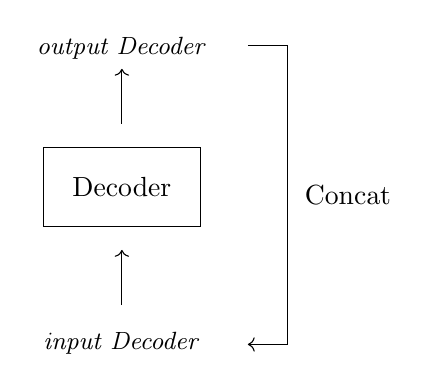
\begin{tikzpicture}
        % Draw arrow from 'input Decoder' to 'output Decoder'
        \draw[->, black] (0, -8) -- (0, -7.3);
        \node[above] at (0, -8.75) {\small{\textit{input Decoder}}};
        
        % Draw rectangle with text 'Decoder'
        \draw[black] (-1,-7) rectangle (1,-6) node[midway] {Decoder};
        
        % Draw arrow from 'output Decoder' to 'input Decoder'
        \draw[->, black] (0, -5.7) -- (0, -5) node[above] {\small{\textit{output Decoder}}};
        
        % Draw curved arrow from 'output Decoder' to 'input Decoder'
        \draw[->, black] (1.6,-4.7) -- (2.1,-4.7) -- (2.1, -8.5) -- (1.6, -8.5);
        \node[right] at (2.2, -6.6) {Concat};
    \end{tikzpicture}
    \caption{Caption}
    \label{ext_teacher_forcing}
\end{figure}

De esta manera, en el ejemplo anterior, el \ti{Decoder} primero recibe en token de iniciación $(t=0)$, luego la secuencia de token de iniciación + \ul{\ti{Ayer}} $(t=1)$, seguido de token de iniciación + \ul{\ti{Ayer}} + \ul{\ti{hizo}} $(t=2)$, etc. Nótese que, debido al token de iniciación, la secuencia está desplazada hacia la derecha. Eso es lo que quiere decir \ti{shifted right} de la figura \ref{outputs}.

El \ti{Decoder} en la \ti{fase de generación de texto} se comporta algo distinto, pues, por motivos obvios, no tiene acceso al texto \ti{real} que debe predecir. La modificación aquí está en que ahora en vez de ir recibiendo los tokens \ti{reales}, lo que va concatenando son los tokens que va prediciendo cada instante $t$.

El otro aspecto importante a cubrir en esta sección es la \B{codificación posicional}. Se puede pensar que el \ti{Decoder}, al ser secuencial, no necesita esta codificación. Pero, sí que la necesita porque, aunque sea secuencial en el sentido de que va generando palabras una a una, según las va generando, va recibiendo concatenaciones de palabras generadas hasta ese momento. Estas palabras que el \ti{Decoder} recibe, las recibe de manera paralela ---de la misma manera que pasaba con el \ti{Encoder}---. Por tanto, la codificación posicional sigue siendo necesaria.

De la misma manera que con el \ti{Encoding}, el vector de \ti{embedding} de cada palabra que va recibiendo el \ti{Decoder}, se suma a su vector posicional. De nuevo, estos vectores se concatenan en una matriz $E'$ de dimensiones $[S', 512]$ siendo $S'$ en número de tokens concatenados en un instante $t_i$ de tiempo.

\subsubsubsection{Enmascaramiento de atención}

\begin{figure}[H]
    \centering
    \includegraphics[scale = 0.7]{imgs/trans_arq_4.png}
    \begin{tikzpicture}[overlay]
        \draw[->, black, ultra thick] (1.5,1.5) -- (-0-.3,1.5);
    \end{tikzpicture}
    \caption{Subcapa de enmascaramiento. \scriptsize{Fuente: \parencite{transformers}}}
    \label{enmcascaramiento}
\end{figure}

El enmascaramiento tiene que ver  con la propiedad que en el \ti{paper} denominan auto-regresiva.  Esto, lo que viene decir es que, para que el modelo genere un texto coherente, cada palabra concatenada que recibe el \ti{Decoder}, no tiene acceso a información de palabras que estén a su derecha en la secuencia, i.e. palabras que hayan sido añadidas a la secuencia después de la palabra en cuestión.

En otras palabras, siguiendo con el ejemplo de antes, \ul{\ti{Ayer hizo mucho frío}}, supóngase que el \ti{Decoder} está prediciendo bien. Hasta ahora ha predicho las palabras \ti{Ayer} e \ti{hizo}. Bien, pues el enmascaramiento, de lo que se va a encargar es que la palabra \ti{Ayer}, no tenga acceso a la información de que la palabra \ti{hizo} se ha añadido a la secuencia, pues está a su derecha en la secuencia. En cambio, \ti{hizo} sí que tiene acceso a la palabra \ti{Ayer}, pues esta la palabra \ti{hizo} está a la derecha de la palabra \ti{Ayer} en la secuencia de \ti{input} del \ti{Decoder}.

En esta subcapa, se genera la matriz $Q$. Es decir, un vector de \ti{búsqueda de características} de cada palabra en la secuencia de \ti{input}. Estos vectores que componen las filas de la matriz $Q$ no son iguales al del \ti{Decoder} por la restricción del enmascaramiento.

\subsubsubsection{Atención Decoder}
\label{atencion_decoder}
\begin{figure}[H]
    \centering
    \includegraphics{imgs/trans_arq_6.png}
    \caption{Atención Decoder. \scriptsize{Fuente: \parencite{transformers}}}
    \label{atencion_decoder}
\end{figure}

El bloque de atención del \ti{Decoder} funciona sutilmente distinto al que se ha visto con anterioridad. Esta subcapa recibe dos \ti{inputs}:
\begin{itemize}
    \item Por una parte, como se ve en la imagen \ref{atencion_decoder}, recibe información de la última capa del \ti{Encoder}. Esta información en concreto, son las matrices $K$ y $V$ de esta capa del \ti{Encoder}. Esto se hace con el motivo de aportar contexto de la palabra que se está procesado (y esto ocurre para las seis capas del \ti{Decoder}). En cierta manera, esto permite que una palabra dada, e.g. \ul{\ti{Ayer}}, aunque no tenga acceso a información de palabras posteriores en su secuencia, el \ti{Decoder} siga teniendo acceso a un contexto global calculado en el \ti{Encoder}. Esta transmisión de información de contexto global por parte del \ti{Encoder} al \ti{Decoder} se denomina \ti{Atención} y es distinto al concepto de \ti{self-attention} (sección \ref{encoder}).
    \item Por otra parte, esta subcapa recibe la matriz $Q$ de la subcapa de enmascaramiento.
\end{itemize}

De esta manera, para  predecir el \ti{output} se hace lo mismo que se ha hecho en el \ti{Encoder}. En este punto, el \ti{Decoder} ya tiene la matrices $Q,K$ y $V$ de dimensiones $[S', 512]$ cada una de ellas. Se multiplican por unas matrices de pesos $W^Q, W^K$ y $W^V$ respectivamente para obtener una matriz $Z$ de dimensión $[S', 64]$. Esta atención se repite $h = 8$ veces para obtener distintos grados de atenciones, y finalmente, al concatenar cada una de las matrices $Z$ de  cada dimensión de atención, se multiplica por otra matriz de pesos $W^O$ de dimensión $[64 \cdot 8, 512]$ para obtener la dimensión consistente de salida $[S', 512]$.

Esta matriz resultado sigue el mismo proceso. Se pasa a un bloque residual que recibe este \ti{input} y el \ti{output} de la subcapa anterior. Luego se pasa por una FFN y posteriormente por otro bloque residual. 

Este proceso se repite $N = 6$ veces, pues hay 6 bloques de \ti{Decoder}.

\subsubsection{Salida de Transformer}

\begin{figure}[H]
    \centering
    \includegraphics{imgs/trans_arq_5.png}
    \caption{Salida de Transformer. \scriptsize{Fuente: \parencite{transformers}}}
    \label{salida}
\end{figure}
Finalmente, la salida de la última capa del \ti{Decoder}, es una matriz de dimensión $[S', 512]$. Dicha matriz se pasa por una función lineal que se va encargar de convertir esta información en un único vector de $D$ dimensiones, siendo $D$ el número de palabras del idioma al que se esté generando el texto. Es decir, que cada posición de este vector, corresponde a una palabra del idioma en cuestión ---este idioma puede ser el mismo que el de la secuencia de entrada si, por ejemplo, la función del \ti{Decoder} es generar un resumen; o por otro lado, puede ser otro idioma si es un problema de traducción de texto---.

Finalmente, este vector se pasa por una función Softmax que pasa los valores de este vector a probabilidades, de tal manera que la suma de todos los valores de este vector sume uno. El output será aquella palabra que corresponda a la posición con mayor probabilidad del vector resultante de aplicar la función Softmax. 
\subsection{Informer}

\subsubsection{Codificación Informer}
\label{ap:codif}

La codificación que hace el Informer en los datos de entrada es bastante completa. Y es que, una peculiaridad que tienen los datos temporales, es que su posición lleva asociado un \ti{time stamp}, el cual indica el minuto, hora, día, mes, etc. en el que el dato se ha recogido ---dependiendo de la serie temporal, los \ti{time stamps} pueden variar entre unos y otros---. Todos estos \ti{time stamps} aportan información adicional que un algoritmo puede exprimir. En este caso, esta información adicional la tiene en cuenta en Informer. 

El Informer, a la hora de codificar los datos de la serie temporal, i.e. procesamiento de los datos para introducirlos en el modelo, hace tres codificaciones distintas; cada una aportando una información distinta al algoritmo. 

% ############# LOS ?? DEJARLOS. LUEGO, AL JUNTARLO CON LA OTRA PARTE ESTARÁ BIEN ##################
\begin{itemize}
    \item Como ya se ha comentado en la sección del Informer  \ref{sec_informer}, el contexto local en series temporales es fundamental. Para aportar esta información local al algoritmo,  Informer \parencite{informer} realiza una codificación fija (\ti{fixed}), de la misma manera  que se hace en el Transformer original, i.e. con senos y cosenos, para la posición de cada uno de los datos en la serie temporal. 
    \item Por otra parte, emplea el \ti{time stamp} para aportar un contexto global. Esto se hace a través de una codificación aprendible (\ti{learnable embedding}). 
    \item Por último, cada dato de la serie temporal se proyecta en un vector de $d_{model}$ dimensiones (mismas dimensiones que los vectores de codificación anteriores) para poder añadir esta información a las dos codificaciones anteriores.
\end{itemize}

Véase la figura \ref{cod_inf} para poder ver esto de una manera más visual.

\begin{figure}[H]
    \centering
    \includegraphics[width = 0.8\textwidth]{imgs/cod_inf.png}
    \caption{Codificación completa del Informer. \scriptsize{Fuente: \parencite{informer}}}.
    \label{cod_inf}
\end{figure}

\subsubsection{Algoritmo ProbSparse}
\label{ap:prob}

Este algoritmo surge de la necesidad de reducir la complejidad con la que se calcula la atención en el Tranformer. La idea intuitiva detrás de \ti{ProbSpare}, es que los autores se dieron cuenta de que sólo algunos productos escalares entre las matrices $Q$ y $K$ proporcionaban la atención más relevante (véase figura \ref{aten_mat}).

\begin{figure}[H]
    \centering
    \includegraphics[scale = 0.5]{imgs/aten_mat.png}
    \caption{Ejemplo matriz de atención. \scriptsize{Fuente: \parencite{rnnPlusAttention}}}
    \label{aten_mat}
\end{figure}

En la figura \ref{aten_mat}, cuanto más clara es una celda, se traduce en un producto escalar entre $q_i$ y $k_j$ con una alta atención. Es fácil ver que, en su gran mayoría, las celdas son más bien oscuras. Esto se puede ver da manera más rigurosa en la figura \ref{long_tail_dist}.

\begin{figure}[H]
    \centering
    \includegraphics[scale = 0.75]{imgs/long_tail_dist.png}
    \caption{Distribución de las atenciones con forma de cola larga. \scriptsize{Fuente: \parencite{informer}}}
    \label{long_tail_dist}
\end{figure}

En la figura \ref{long_tail_dist} se puede ver cómo solamente hay unos pocos productos escalares entre los vectores $q_i$ y $k_j$ que aportan una alta atención ---i.e. un valor de softmax alto---. Un producto escalar con una atención alta induce a que la distribución del vector $q_i$ asociado a dicho producto escalar sea muy diferente a una distribución uniforme \parencite{informer}. Esto es porque si un vector $q_i$ sigue una distribución uniforme, se traduce en que no \ti{busca} prestar atención a ningún dato en la secuencia en concreto, y por ende se puede no tener en cuenta para computar la atención. 


Para determinar si la distribución de un vector $q_i$ sigue una distribución que se asemeja a una distribución uniforme, se emplea la divergencia de Kullback-Leibler \parencite{KL}. Aunque su explicación va más allá del contenido de este trabajo, basta con saber que cuanto mayor sea $q_i$, más discrepancia hay entre su distribución y la distribución uniforme; lo que implica que dicho vector $q_i$ es relevante a la hora de calcular la atención. A este proceso se le denomina \ti{Query Sparsity Measurement} y está recogido en $M$ en la figura \ref{probSparse}.

Como el objetivo es reducir la complejidad de la atención del Transformer original, seleccionando los $q_i$ con mayor importancia no es suficiente, pues para calcular estos, hay que realizar el producto escalar entre $Q$ y $K$, lo cual sigue siendo manteniendo la misma complejidad ($\mathcal{O}(L ^2)$). Para ello, se seleccionan $U$ vectores aleatorios $k_j$ de la matriz $K$. Esta muestra se considera representativa. En la figura \ref{probSparse} se puede ver un pseudo código de estos pasos recientemente explicados.
\begin{figure}[H]
    \centering
    \includegraphics{imgs/probSparse.png}
    \caption{Pseudo-código algoritmo. \scriptsize{Fuente: \parencite{informer}}.}
    \label{probSparse}
\end{figure}

En el paso 2), se seleccionan $U$ vectores aleatorios de $K$. Por lo general, $m$ y $n$ suelen ser ambos iguales: la longitud de la secuencia de entrada denotada como $L$. Por tanto se seleccionan $L \ln L$ vectores aleatorios de $K$. Con esto, se puede calcular $M$ y seleccionar los $u$ vectores $q_i$ que más discrepancia tengan con una distribución uniforme ---i.e. lo que tengan un valor más alto---. Con esto se consigue reducir la complejidad del cálculo de la atención de ($\mathcal{O}(L ^2)$) a $\mathcal{O}(L \ln L$).

Cabe remarcar que el Informer mantiene la \ti{Multi-head Attention} del Transformer original; lo que implica que el algoritmo de la figura \ref{probSparse} se calcula varias veces por cada capa de atención, evitando de esta manera información redundante, y obteniendo distintos vectores $q \in \overline{Q}$, así como distintos vectores aleatorios $k \in \overline{K}$.

\subsubsection{Comparativa Informer}
\label{ap:inf_res}

Se muestra una tabla que compara el Informer con algunos algoritmos estado del arte hasta la fecha: LogTrans(i.e. LogSparse) \parencite{logSparse}, Reformer \parencite{reformer}, LSTMa\fnm\ \parencite{rnnPlusAttention}, DeepAR \parencite{deepAR}, ARIMA \parencite{ARIMA}, Prophet \parencite{Prophet}.
\fnt{RNN + atención.}

\begin{figure}[H]
    \centering
    \includegraphics[scale = 0.65]{imgs/informer_results.png}
    \caption{Tabla comparativa Informer. \scriptsize{Fuente: \parencite{informer}}}
    \label{inf_results}
\end{figure}

\begin{nota}
    El Informer$^{\dag}$ de la segunda columna de la tabla \ref{inf_results} es la arquitectura del informer sin haber modificado la atención, i.e. sin haber aplicado el algoritmo de \ti{ProbSparse}.
\end{nota}
\end{comment}


%\clearpage
%\thispagestyle{empty}
%\printindex \nocite{*}
%\appendix
\pagestyle{plain}

\section*{Cosas a comentar}


\begin{comment}
    \textsuperscript{\hyperref[ap:tfa]{A15}}
\end{comment}

\begin{atencion}
    Poner transformers con cursiva
\end{atencion}

% REFERENCIAS
\newpage{\pagestyle{empty}}
\addcontentsline{toc}{section}{Referencias}
%https://github.com/SantiPlanet/apalike

\printbibliography[title = {Referencias}]





\end{document}
